% Instituto Nacional de Pesquisas Espaciais - INPE
% https://github.com/cfbastarz/EstiloBeamerINPE
% V1.2
% carlos.bastarz@inpe.br (15/04/2021)

\documentclass[10pt,aspectratio=169]{beamer}

% Tema padrão (base)
\usetheme{default}
%\usetheme{Singapore}
%\usetheme{Boadilla}
%\usetheme{minflat}

% Carregamento dos pacotes utilizados
\usepackage[brazilian]{babel} % comentar este pacote se a apresentação for em inglês
\usepackage{times}

%\usepackage[utf8]{inputenc}
\usepackage{fontspec}

\usepackage{graphicx}
\usepackage{subfigure}

\usepackage{tabularx}
\usepackage{booktabs}
\usepackage{hyperref}

\usepackage[alf]{abntex2cite}
\usepackage{bibentry}

\usepackage{fontawesome5}

\usepackage[skins,theorems]{tcolorbox}
\usepackage{pst-all}
\usepackage{tikz}
\usetikzlibrary{decorations.pathreplacing}
\usepackage{pifont}
\usetikzlibrary{positioning}
\usetikzlibrary{arrows}

\usepackage[absolute,overlay]{textpos}

\usepackage{pst-all}
\usetikzlibrary{positioning}
\usepackage{pgfplots}
\usepackage{textcomp}
\usepgfplotslibrary{dateplot}


\usepackage{pifont}
\newcommand{\itemcolor}[1]
{
  \renewcommand{\makelabel}[1]{\color{#1}\hfil ##1}
}
  
\definecolor{myblack}{RGB}{0,0,0}
\definecolor{mygrey}{RGB}{204,204,204}
\definecolor{mydarkgrey}{RGB}{152,152,152}
\definecolor{mygreen}{RGB}{34,55,58}
\pgfplotsset{width=4.5cm,compat=1.8,every tick label/.append style={font=\tiny}}
\pgfmathdeclarefunction{gauss}{2}{%
\pgfmathparse{1/(#2*sqrt(2*pi))*exp(-((x-#1)^2)/(2*#2^2))}%
}

\newcommand{\unilogo}{
  \setlength{\TPHorizModule}{1pt}
  \setlength{\TPVertModule}{1pt}
   % textblock{}{x,y}: pos(x) = leftUpperCorner + (x * \TPHorizModule), pos(y) = leftUpperCorner - (y * \TPVertModule)
  \begin{textblock}{1}(25,2)
    
\includegraphics[width=45pt,height=45pt]{Logomarca2020.png}
  \end{textblock}
  } 

%%%%%%%%%%%%%%%%

\tikzstyle{process1} = [rectangle, rounded corners, minimum width=3cm, minimum height=1cm, text centered, draw=black, fill=MaterialBlue!30]

\tikzstyle{process2} = [rectangle, rounded corners, minimum width=3cm, minimum height=1cm, text centered, draw=black, fill=MaterialYellow!30]

\tikzstyle{process3} = [rectangle, rounded corners, minimum width=3cm, minimum height=1cm, text centered, draw=black, fill=MaterialGrey!30]

\tikzstyle{process4} = [rectangle, rounded corners, minimum width=3cm, minimum height=1cm, text centered, draw=black, fill=MaterialOrange!30]

\tikzstyle{process5} = [rectangle, rounded corners, minimum width=3cm, minimum height=1cm, text centered, draw=black, fill=MaterialGreen!30]

\tikzstyle{process6} = [rectangle, rounded corners, minimum width=3cm, minimum height=1cm, text centered, draw=black, fill=MaterialRed!30]

\tikzstyle{process7} = [rectangle, rounded corners, minimum width=3cm, minimum height=1cm, text centered, draw=black, fill=MaterialPurple!30]

\tikzstyle{process8} = [rectangle, rounded corners, minimum width=3cm, minimum height=1cm, text centered, draw=black, fill=MaterialCyan!30]

\tikzstyle{arrow} = [thick,->,>=stealth]      

\setbeamerfont{framesubtitle}{size=\large}

%%%%%%%%%%%%%%%%%%%%%%%%%%%%%%%%%%%%%%%%%%%%%%%
% DEFINIÇÃO DO TEMA

% Definiçãoo do estilo das fontes
\usefonttheme[onlymath]{serif}
\usefonttheme{professionalfonts} % using non standard fonts for beamer
\usefonttheme{serif} % default family is serif
\usepackage{fontspec}
%\setmainfont{Liberation Sans}

% Imagem de fundo dos frames
\usebackgroundtemplate{%
	
\includegraphics[width=\paperwidth,height=\paperheight]{fundo_slide_inpe_sem_logo.png}%
	}

% Selo de 60 anos do INPE (comentar a linha abaixo caso não queira utilizar)
%\titlegraphic{
\includegraphics[scale=0.15]{60Anosfinal.png}\vspace*{-50pt}}
\titlegraphic{
\includegraphics[scale=0.25]{logo_monan_pequeno.png}\vspace*{-50pt}}

\logo{\unilogo}

% Remove a barra de navegação dos frames
\beamertemplatenavigationsymbolsempty

% Rodapé dos frames
\makeatother
\setbeamertemplate{footline}
{
	\leavevmode%
	\hbox{%
	\begin{beamercolorbox}[wd=.35\paperwidth,ht=2.25ex,dp=1ex,left]{author in head/foot}%
		\hspace*{13ex}\usebeamerfont{author in head/foot}\insertshortauthor
	\end{beamercolorbox}%
	\begin{beamercolorbox}[wd=.65\paperwidth,ht=2.25ex,dp=1ex,right]{title in head/foot}%
		\usebeamerfont{title in head/foot}\insertshorttitle\hspace*{3em}
		\insertframenumber{} / \inserttotalframenumber\hspace*{3ex}
	\end{beamercolorbox}}%
	\vskip4pt%
}
\makeatletter

% Insere o TOC com números (seções e subseções)
\setbeamertemplate{section in toc}[sections numbered]
\setbeamertemplate{subsection in toc}[subsections numbered]

% Definição das cores do tema
\definecolor{azulinpe}{RGB}{0, 110, 175}
\definecolor{laranjainpe}{RGB}{248, 133, 31}
\definecolor{verdeinpe}{RGB}{73, 119, 28}

\setbeamercolor{title}{fg=azulinpe}
\setbeamercolor{frametitle}{fg=azulinpe, bg=laranjainpe}

\setbeamercolor{palette primary}{fg=azulinpe}
\setbeamercolor{palette secondary}{fg=azulinpe}
\setbeamercolor{palette tertiary}{fg=azulinpe}
\setbeamercolor{palette quaternary}{fg=azulinpe}

\setbeamercolor{structure}{fg=azulinpe} % itemize, enumerate, etc
\setbeamercolor{section in toc}{fg=azulinpe} % TOC sections

% Títulos dos frames
\makeatletter
\defbeamertemplate*{frametitle}{mydefault}[1][left]
{
  \ifbeamercolorempty[bg]{frametitle}{}{\nointerlineskip}%
  \@tempdima=\textwidth%
  \advance\@tempdima by\beamer@leftmargin%
  \advance\@tempdima by\beamer@rightmargin%
  \hspace{1.3cm}
  %
\includegraphics[scale=0.75]{barra_secao.png}
  \hspace{-0.5cm}
  \pgfsetfillopacity{0}
  \begin{beamercolorbox}[sep=0.3cm,#1,wd=0.64\textwidth]{frametitle}
    \usebeamerfont{frametitle}%
    \vbox{}\vskip-1ex%
    \if@tempswa\else\csname beamer@fte#1\endcsname\fi%
    \strut\pgfsetfillopacity{1}\insertframetitle\strut\par%
    {%
      {\usebeamerfont{framesubtitle}\usebeamercolor[fg]{framesubtitle}\insertframesubtitle\strut\par}%
    }%
    \vskip-1ex%
    \if@tempswa\else\vskip-.3cm\fi% set inside beamercolorbox... evil here...
  \end{beamercolorbox}%
}
\makeatother

% Blocos customizados
\newenvironment<>{problock1}[1]{%
  \begin{actionenv}#2%
      \def\insertblocktitle{#1}%
      \par%
      \mode<presentation>{%
        \setbeamercolor{block title}{fg=laranjainpe, bg=azulinpe}
      \setbeamercolor{block body}{fg=azulinpe, bg=white}
      \setbeamercolor{itemize item}{fg=laranjainpe}
      \setbeamertemplate{itemize item}[triangle]
     }%
      \usebeamertemplate{block begin}}
    {\par\usebeamertemplate{block end}\end{actionenv}}

\newenvironment<>{problock2}[1]{%
  \begin{actionenv}#2%
      \def\insertblocktitle{#1}%
      \par%
      \mode<presentation>{%
        \setbeamercolor{block title}{fg=azulinpe, bg=laranjainpe}
      \setbeamercolor{block body}{fg=laranjainpe, bg=white}
      \setbeamercolor{itemize item}{fg=azulinpe}
      \setbeamertemplate{itemize item}[triangle]
     }%
      \usebeamertemplate{block begin}}
    {\par\usebeamertemplate{block end}\end{actionenv}}


\setbeamertemplate{caption}{\insertcaption} 

\hypersetup{colorlinks,linkcolor=,citecolor=,urlcolor=azulinpe,backref=true}

\newcommand{\nologo}{\setbeamertemplate{logo}{}}

%%%%%%%%%%%%%%%%%%%%%%%%%%%%%%%%%%%%%%%%%%%%%%%


% Informações da capa da apresentação
\title{Matriz de Covariâncias dos Erros de Previsão (Matriz $\mathbf{B}$)}
\author{Carlos Frederico Bastarz\\ \href{https://github.com/cfbastarz}{\faGithub} \href{http://lattes.cnpq.br/2410960909883784}{\faGraduationCap} \href{https://www.researchgate.net/profile/Carlos_Bastarz}{\faResearchgate} \href{mailto:carlos.bastarz@inpe.br}{\faEnvelope}}
\institute{\textbf{\small{Workshop DIMNT}\\\vspace{0.5em}\footnotesize{``A Assimilação de Dados nas Componentes do Sistema Terrestre:\\Status e Perspectivas Futuras no Contexto do MONAN''}}}
\date{
	%\today 
	06 de outubro de 2022
}

% A partir daqui inicia-se o documento
\begin{document}

% Capa (NÃO MODIFICAR)
{
\setbeamertemplate{footline}{} 
\begin{frame}
	\vspace{1cm}
	\titlepage
\end{frame}
}
 
% Reinicia do contador dos frames 
\addtocounter{framenumber}{-1}
 
% Sumário
% \begin{frame}{Sumário}
% 	\tableofcontents
% \end{frame}

\begin{frame}
    \frametitle{Sumário}
    \framesubtitle{\faListOl}
    \begin{textblock}{15}(1.5,4)
        \begin{columns}[t]
            \begin{column}{.5\textwidth}
                \large\tableofcontents[sections={1-3}]
            \end{column}
            \begin{column}{.5\textwidth}
                \large\tableofcontents[sections={4-6}]
            \end{column}
        \end{columns}
    \end{textblock}    
\end{frame}

\section{Introdução}

\subsection{Um Desafio}

\begin{frame}[fragile]{Introdução}
\framesubtitle{Um Desafio}
  %\onslide<1->
  Fontes de incerteza são uma característica intrínseca a qualquer sistema dinâmico.\\
  %\onslide<2->
  \begin{columns}[onlytextwidth,T]
    \column{\dimexpr\linewidth-43mm-5mm}
      \parbox{\linewidth}
      {\vspace{0.4cm} 
        Na década de 1960, Edward N. Lorenz mostrou que a atmosfera possui previsibilidade de duas semanas.
      } \hfill
    \column{24mm}
      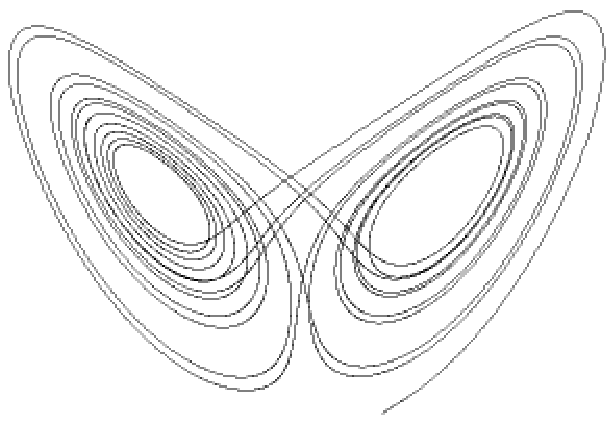
\includegraphics[scale=0.27]{figs/lorenz_attractor.pdf} \hfill
    \column{12mm}
      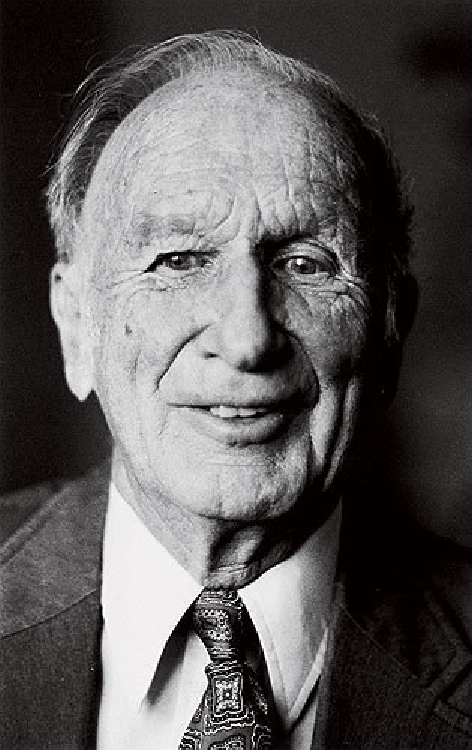
\includegraphics[scale=0.15]{figs/lorenz.pdf} 
  \end{columns}
  %\onslide<3->
  \pause
%  \metroset{block=fill}
  \begin{block}{Um Desafio:}
    \vspace{0.5em}
    Como fazer com que os modelos atuais possam prever bem dentro deste limite (e além dele)?
  \end{block}
\end{frame}

\subsection{Modelagem e Assimilação}

%\begin{frame}[fragile]{Introdução}
%\framesubtitle{Modelagem e Assimilação}
%\vspace{1em}
%  Os modelos de PNT são realizados dentro de uma estrutura de modelagem que compreende:
%  \begin{columns}
%    \column{0.45\textwidth}  
%      \vbox to 0.5\textheight{
%        %\vfill
%        \vspace{11em}
%        %\hspace{-0.5cm}
%        \scalebox{0.9}{
%          \begin{tikzpicture}[overlay,baseline=(current bounding box.north)]
%            \newcommand{\CircleA}
%            {
%              \draw (2,2) circle (1cm) node [left] {\tiny Modelo};
%            }
%            \newcommand{\CircleB}
%            {
%              \draw (3,2) circle (1cm) node [right] {\tiny Obs.};
%            }
%            \newcommand{\CircleC}
%            {
%              \draw (2.5,1) circle (1cm) node [below] {\tiny AD};
%            }
%            \newcommand{\Intersect}
%            {
%              \begin{scope}
%                \clip (2,2) circle (1cm);
%                \clip (3,2) circle (1cm);
%                \clip (2.5,1) circle (1cm);
%                \draw[fill=laranjainpe](2.5,1) circle (1cm);
%              \end{scope}
%            }
%            \newcommand{\Arrow}
%            {
%              \draw [->,>=stealth] (2.5,1.65) -- (3.8,0.97) node [right] {\tiny Boa Análise!};
%            }
%            \only<2-> \CircleA
%            \only<3-> \CircleB
%            \only<4-> \CircleC
%            \only<5-> \Intersect
%            \only<6-> \Arrow
%          \end{tikzpicture} 
%        }
%      }
%    \column{0.4\textwidth}
%      \onslide<6-> 
%      %\vspace{-1.5cm}
%      \hspace{0.75cm}
%      \scalebox{0.75}{
%        \begin{tikzpicture}[overlay,baseline=(current bounding box.north)]
%          \draw (0.25,2) ellipse (1.5cm and 0.5cm) node {\tiny Observações (+/-3h)};
%          \draw (3.75,2) ellipse (1.5cm and 0.5cm) node {\tiny Previsão de Curto Prazo};
%          \draw (0.5,0.5) rectangle node [align=center] {\tiny Análise global \\ \tiny (Interpolação Estatística)} (3.5,-0.5);
%          \draw [->,>=stealth] (0,1.5) -- (1.5,0.5);
%          \draw [->,>=stealth] (4,1.5) -- (2.5,0.5);
%          \draw [->,>=stealth] (2,-0.5) -- node[fill opacity=1,fill=white] {\tiny Condição Inicial} (2,-1.5);
%          \draw (0.5,-1.5) rectangle node [align=center] {\tiny Modelo de PNT Global} (3.5,-1.95);
%          \draw (3,-1.95) -- node[fill opacity=1,fill=white] {\tiny Previsão 6h} (3,-3);
%          \draw (3,-3) -- (4.5,-3);
%          \draw [->,>=stealth] (4.5,-3) -- (4.5,1.54);
%          \draw [densely dotted,->,>=stealth] (1.5,-1.95) -- (1,-3) node [below] {\tiny Previsão Operacional};
%        \end{tikzpicture}    
%      }
%  \end{columns} 
%  %\vspace{0.75cm}
%  \onslide<7>
%  \begin{block}{Modelagem e Assimilação:}
%    Uma vez estabelecido o processo de modelagem, as fontes de incerteza devem ser abordadas para que o seu impacto seja mínimo.
%  \end{block}
%\end{frame}

\begin{frame}[fragile]{Introdução}
\framesubtitle{Modelagem e Assimilação}
%\vspace{1em}
  Os modelos de PNT são realizados dentro de uma estrutura de modelagem que compreende:
  \begin{columns}
    \column{0.45\textwidth}  
      \vbox to 0.5\textheight{
        %\vfill
        \vspace{14em}
        \hspace*{-3em}
        \scalebox{1.5}{
          \begin{tikzpicture}[overlay,baseline=(current bounding box.north)]
            \newcommand{\CircleA}
            {
              \draw (2,2) circle (1cm) node [left] {\tiny Modelo};
            }
            \newcommand{\CircleB}
            {
              \draw (3,2) circle (1cm) node [right] {\tiny Obs.};
            }
            \newcommand{\CircleC}
            {
              \draw (2.5,1) circle (1cm) node [below] {\tiny AD};
            }
            \newcommand{\Intersect}
            {
              \begin{scope}
                \clip (2,2) circle (1cm);
                \clip (3,2) circle (1cm);
                \clip (2.5,1) circle (1cm);
                \draw[fill=verdeinpe](2.5,1) circle (1cm);
              \end{scope}
            }
            \newcommand{\Arrow}
            {
              \draw [->,>=stealth] (2.5,1.65) -- (3.8,0.97) node [right] {\tiny Boa Análise!};
            }
            \only<2-> \CircleA
            \only<3-> \CircleB
            \only<4-> \CircleC
            \only<5-> \Intersect
            \only<6-> \Arrow
          \end{tikzpicture} 
        }
      }
    \column{0.55\textwidth}
      \onslide<6-> 
%      %\vspace{-1.5cm}
%      \hspace{0.75cm}
%      \scalebox{0.75}{
%        \begin{tikzpicture}[overlay,baseline=(current bounding box.north)]
%          \draw (0.25,2) ellipse (1.5cm and 0.5cm) node {\tiny Observações (+/-3h)};
%          \draw (3.75,2) ellipse (1.5cm and 0.5cm) node {\tiny Previsão de Curto Prazo};
%          \draw (0.5,0.5) rectangle node [align=center] {\tiny Análise global \\ \tiny (Interpolação Estatística)} (3.5,-0.5);
%          \draw [->,>=stealth] (0,1.5) -- (1.5,0.5);
%          \draw [->,>=stealth] (4,1.5) -- (2.5,0.5);
%          \draw [->,>=stealth] (2,-0.5) -- node[fill opacity=1,fill=white] {\tiny Condição Inicial} (2,-1.5);
%          \draw (0.5,-1.5) rectangle node [align=center] {\tiny Modelo de PNT Global} (3.5,-1.95);
%          \draw (3,-1.95) -- node[fill opacity=1,fill=white] {\tiny Previsão 6h} (3,-3);
%          \draw (3,-3) -- (4.5,-3);
%          \draw [->,>=stealth] (4.5,-3) -- (4.5,1.54);
%          \draw [densely dotted,->,>=stealth] (1.5,-1.95) -- (1,-3) node [below] {\tiny Previsão Operacional};
%        \end{tikzpicture}    
%      }
	\vspace{2em}
  \begin{block}{Modelagem e Assimilação:}
  \vspace{0.5em}
   Uma vez estabelecido o processo de modelagem, as fontes de incerteza devem ser abordadas para que o seu impacto seja mínimo.
  \end{block}
  \end{columns} 
%  %\vspace{0.75cm}
%  \onslide<7>
%  \begin{block}{Modelagem e Assimilação:}
%    Uma vez estabelecido o processo de modelagem, as fontes de incerteza devem ser abordadas para que o seu impacto seja mínimo.
%  \end{block}
\end{frame}


\subsection{Fontes de Incerteza}

\begin{frame}[fragile]{Introdução}
\framesubtitle{Fontes de Incerteza}
  %\onslide<1->  
  \begin{block}{Função Custo Variacional Tridimensional (3DVar):}
  \vspace{0.5em}
  Em geral, as fontes de incerteza do processo de modelagem são representadas por:
  %\onslide<2->  
  \begin{itemize}
    \item Modelo (eg., dinâmica e física);
    \onslide<3->
    \item Observações (eg., medição, instrumento, grau de processamento);
    \onslide<4->
    \item Assimilação de Dados (eg., operadores de observação, modelos adjunto e tangente linear, tamanho conjunto).
  \end{itemize}
  %\onslide<5->
  \pause
  \vspace{0.5em}
  Na AD, estes erros são modelados em matrizes de covariâncias que tratam das relações espaço-temporais entre as quantidades observadas e diagnosticadas/prognosticadas.
\end{block}
  \vspace{0.5cm}
  
%   \onslide<6->  
% %  \metroset{block=fill}
%   \begin{block}{Função Custo Variacional Tridimensional (3DVar):}
%     \vspace{1em}
%     \centering
%     \only<6>{$J(\mathbf{x}) = \frac{1}{2} (\mathbf{x} - \mathbf{x}^{b})^{T} \mathbf{B}^{-1} (\mathbf{x} - \mathbf{x}^{b}) + \frac{1}{2} [\mathbf{y}^{o} - {\mathbf{H}}(\mathbf{x})]^{T} \mathbf{R}^{-1} [\mathbf{y}^{o} - {\mathbf{H}}(\mathbf{x})]$}
%     \only<7>{$J(\mathbf{x}) = \frac{1}{2} (\mathbf{x} - \mathbf{x}^{b})^{T} {\color{red}{\mathbf{B}^{-1}}} (\mathbf{x} - \mathbf{x}^{b}) + \frac{1}{2} [\mathbf{y}^{o} - {\color{green}{\mathbf{H}}}(\mathbf{x})]^{T} {\color{blue}{\mathbf{R}^{-1}}} [\mathbf{y}^{o} - {\color{green}{\mathbf{H}}}(\mathbf{x})]$}
%     \only<8>{$J(\mathbf{x}) = \underbrace{ \frac{1}{2} (\mathbf{x} - \mathbf{x}^{b})^{T} {\color{red}{\mathbf{B}^{-1}}} (\mathbf{x} - \mathbf{x}^{b}) } _{J_{b}} + \underbrace{  \frac{1}{2} [\mathbf{y}^{o} - {\color{green}{\mathbf{H}}}(\mathbf{x})]^{T} {\color{blue}{\mathbf{R}^{-1}}} [\mathbf{y}^{o} - {\color{green}{\mathbf{H}}}(\mathbf{x})] }_{J_{o}}$}    
%   \end{block}
  
\end{frame}

\section{Importância da Matriz $\mathbf{B}$}

\subsection{Distribuição Gaussiana dos erros}

\begin{frame}[fragile]{Importância da Matriz $\mathbf{B}$}
\framesubtitle{Distribuição Gaussiana dos Erros}
  \onslide<1->
  \begin{block}{Suposição - Distribuição Gaussiana:}
    \begin{columns}
      \begin{column}{0.4\textwidth}
      	\begin{center}
           \begin{tikzpicture}[scale=1.25]
             \begin{axis}[every axis plot post/.append style={
             mark=none,domain=-2:3,samples=50,smooth},
             % All plots: from -2:2, 50 samples, smooth, no marks
            axis x line*=bottom, % no box around the plot, only x and y axis
            axis y line*=left, % the * suppresses the arrow tips
            enlargelimits=upper]%,% extend the axes a bit to the right and top
            \addplot[style={ultra thick, azulinpe}]{gauss(0,0.5)};
            \addplot[style={ultra thick}, laranjainpe]{gauss(1,0.75)};
          \end{axis}
        \end{tikzpicture}     
      \end{center}   
    \end{column}
    \begin{column}{0.6\textwidth}  %%<--- here
      \begin{center}
      \vspace{-3em}
	\begin{equation*}
	 f(x) = \frac{1}{\sigma\sqrt{2\pi}}e^{-\frac{1}{2}{\big(\frac{x-\mu}{\sigma}\big)^2}}
	\end{equation*}
	\color{azulinpe}{\boldmath{$\mu=0$, $\sigma=0,5$}}\\
	\color{laranjainpe}{\boldmath{$\mu=1$, $\sigma=0,75$}}
	\color{black}{
	\begin{gather*}
		P_{b}(\mathbf{x} - \mathbf{x}_b) \propto e^{\big[\,-\frac{1}{2}(\mathbf{x}-\mathbf{x}_b)^{T}\mathbf{B}^{-1}(\mathbf{x}-\mathbf{x}_b)\big]\,} \\
		\mathbf{B} = \langle(\mathbf{x}_b - \mathbf{x}_t)(\mathbf{x}_b - \mathbf{x}_t)^{T}\rangle
	\end{gather*}
	}
      \end{center}
    \end{column}
  \end{columns}
  \end{block}    
  \onslide<2->
  \begin{block}{Função Custo Variacional Tridimensional (3DVar):}
    \vspace{1em}
    \centering
    \only<2>{$J(\mathbf{x}) = \frac{1}{2} (\mathbf{x} - \mathbf{x}^{b})^{T} \mathbf{B}^{-1} (\mathbf{x} - \mathbf{x}^{b}) + \frac{1}{2} [\mathbf{y}^{o} - {\mathbf{H}}(\mathbf{x})]^{T} \mathbf{R}^{-1} [\mathbf{y}^{o} - {\mathbf{H}}(\mathbf{x})]$}
    \only<3>{$J(\mathbf{x}) = \frac{1}{2} (\mathbf{x} - \mathbf{x}^{b})^{T} {\color{laranjainpe}{\mathbf{B}^{-1}}} (\mathbf{x} - \mathbf{x}^{b}) + \frac{1}{2} [\mathbf{y}^{o} - {\color{verdeinpe}{\mathbf{H}}}(\mathbf{x})]^{T} {\color{azulinpe}{\mathbf{R}^{-1}}} [\mathbf{y}^{o} - {\color{verdeinpe}{\mathbf{H}}}(\mathbf{x})]$}
    \only<4>{$J(\mathbf{x}) = \underbrace{ \frac{1}{2} (\mathbf{x} - \mathbf{x}^{b})^{T} {\color{laranjainpe}{\mathbf{B}^{-1}}} (\mathbf{x} - \mathbf{x}^{b}) } _{J_{b}} + \underbrace{  \frac{1}{2} [\mathbf{y}^{o} - {\color{verdeinpe}{\mathbf{H}}}(\mathbf{x})]^{T} {\color{azulinpe}{\mathbf{R}^{-1}}} [\mathbf{y}^{o} - {\color{verdeinpe}{\mathbf{H}}}(\mathbf{x})] }_{J_{o}}$}    
  \end{block}  
  
\end{frame}

%\subsection{Onde está a Matriz $\mathbf{B}$?}
\subsection{Incremento de Análise}

\begin{frame}[fragile]{Importância da Matriz $\mathbf{B}$}
\framesubtitle{Incremento de Análise}
  \begin{block}{Equação de Análise:}
  \vspace{0.5em}
    Quando $\nabla_{\mathbf{x}}{J(\mathbf{x})} = 0 \Rightarrow \mathbf{x} = \mathbf{x}^{a}$, a função custo variacional resolve essencialmente o mesmo problema que a Interpolação Ótima:
    \begin{equation*}
      \mathbf{x}^{a} = \mathbf{x}^{b} + (\mathbf{B}^{-1} + \mathbf{H}^{T}\mathbf{R}^{-1}\mathbf{H})^{-1}(\mathbf{H}^{T}\mathbf{R}^{-1})[\mathbf{y}^{o} - H(\mathbf{x}^{b})]
    \end{equation*}
  \end{block}
  \pause
    \begin{block}{Aplicação do Incremento de Análise:}  
    \vspace{-0.5em}
    %Considerando uma única observação:
    \begin{equation*}
      \mathbf{H}=[0,\dots,0,1,0,\dots,0] 
    \end{equation*}
    \begin{equation*}
      \mathbf{x}^{a} = \mathbf{x}^{b} + (\mathbf{B}^{-1} + \mathbf{H}^{T}\mathbf{R}^{-1}\mathbf{H})^{-1}(\mathbf{H}^{T}\mathbf{R}^{-1})[\mathbf{y}^{o} - \mathbf{H}(\mathbf{x}^{b})] 
    \end{equation*}
    \begin{equation*}
      \mathbf{x}^{a} - \mathbf{x}^{b} = \frac{\mathbf{B}\mathbf{H}^{T}[\mathbf{y}^{o} - \mathbf{H}(\mathbf{x}^{b})]}{\mathbf{R} + \mathbf{H}\mathbf{B}\mathbf{H}^{T}} 
    \end{equation*}
    \begin{equation*}
      \mathbf{x}^{a}-\mathbf{x}^{b} \propto \mathbf{BH}^{T}
    \end{equation*}
  \end{block}
\end{frame}

\begin{frame}[fragile]{Importância da Matriz $\mathbf{B}$}
\framesubtitle{Incremento de Análise}
    \vspace{-1.5em}
    \begin{figure}[H]
      \centering
    %   \includegraphics[scale=0.09]{./figs/matrizB/incrementos_anl/incremento_analise_bcptec-crop.png}
      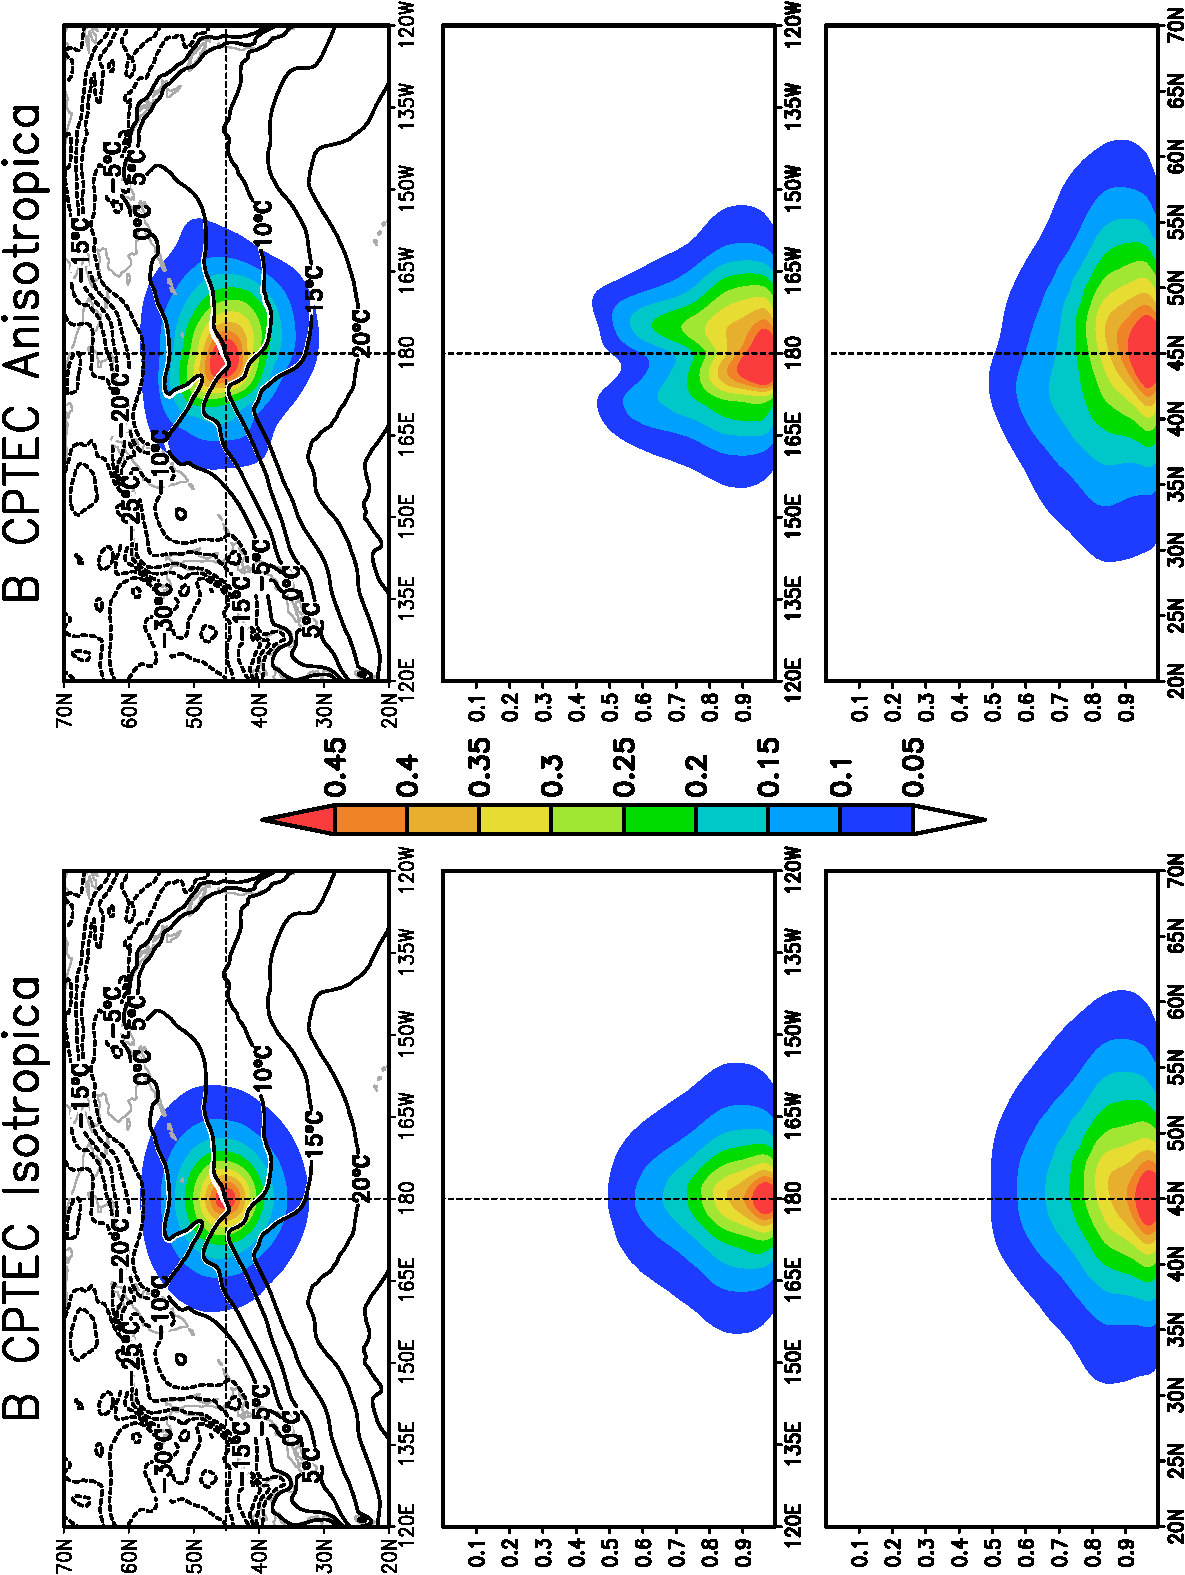
\includegraphics[trim={0.9cm
      0 13cm 14.25cm},clip,scale=1.,angle=-90]{./figs/incr_anl_t1000_Bcptec-artigo_rbmet-crop.pdf}
      \caption{Incremento de uma observação de temperatura.}
    \end{figure}
\end{frame}

\section{Cálculo da Matriz $\mathbf{B}$}

\subsection{Aspecto da Matriz $\mathbf{B}$}

\begin{frame}[fragile]{Cálculo da Matriz $\mathbf{B}$}
\framesubtitle{Aspecto da Matriz $\mathbf{B}$}
  \vspace{-2em}
  \begin{columns}
    \begin{column}{0.5\textwidth}
      %\begin{block}{Aspecto idealizado da Matriz $\mathbf{B}$:}
        \begin{figure}[H]
          \centering
          \hspace*{2em}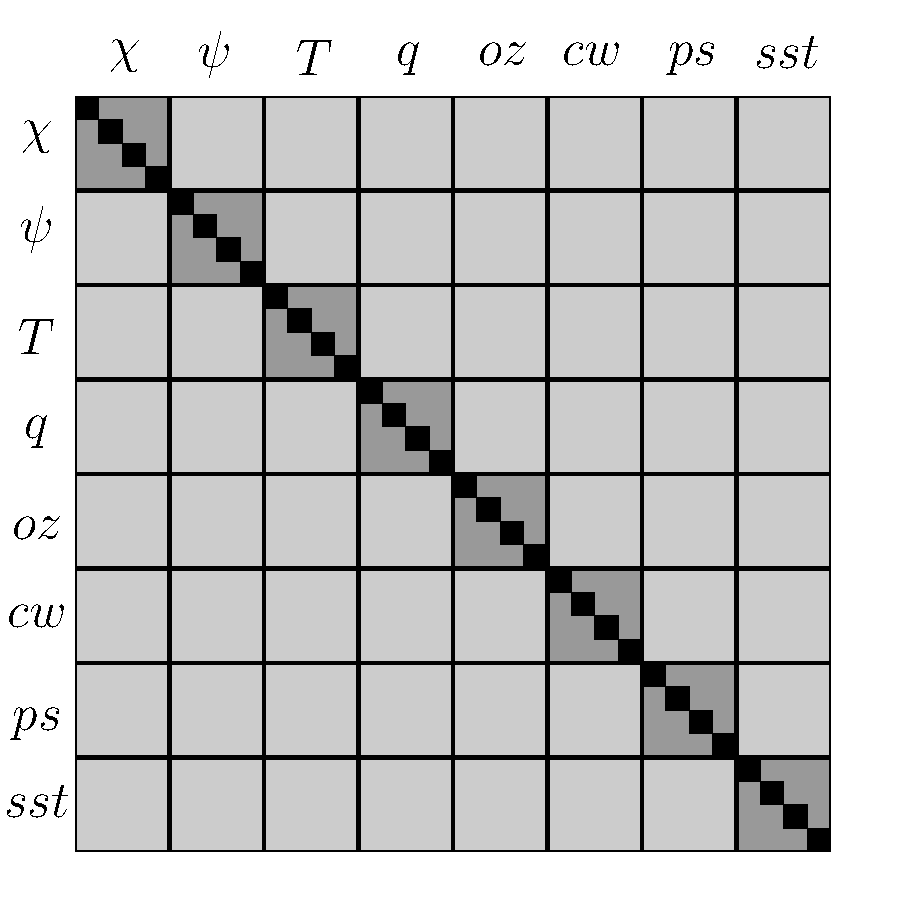
\includegraphics[scale=0.45]{figs/matriz_B-new.pdf}
          \vspace{-1.5em}
          \caption{}
        \end{figure}  
      %\end{block}
    \end{column}
    \begin{column}{0.5\textwidth} 
    %   {\tiny
        \begin{dinglist}{110}
          \itemcolor{myblack}
            \item Variâncias;
          \itemcolor{mygrey}
            \item Covariâncias;
          \itemcolor{mydarkgrey}    
            \item Autocovariâncias.
        \end{dinglist}
    %   }
      \vspace{1em}
      \begin{itemize}
        \item Função de Corrente ($\psi$);     
        \item Velocidade potencial ($\chi$);
        \item Temperatura absoluta ($T$);
        \item Pressão em superfície ($ps$);
        \item Ozônio ($oz$);
        \item Conteúdo de água líquida ($cw$);
        \item Temperatura da superfície do mar ($sst$).
      \end{itemize}
    \end{column}
  \end{columns}
\end{frame}

\subsection{Método NMC}

%\begin{frame}[fragile]{Cálculo da Matriz $\mathbf{B}$}
%\framesubtitle{Método NMC}
%%  \metroset{block=fill}
%  \begin{block}{Método NMC \cite{parrishetal/1992}:}
%    \setbeamercovered{transparent}
%    \begin{itemize}
%      \item Preconiza que as correlações espaciais dos erros do modelo são semelhantes às correlações entre as previsões de 48 e 24 horas;
%      \pause \item Amplamente utilizado e aplicado em métodos variacionais;
%      \pause \item Facilidade de acesso aos pares de previsões de 48 e 24 horas.
%    \end{itemize}  
%  \end{block}
%\end{frame}

%\begin{frame}[fragile]{Cálculo da Matriz $\mathbf{B}$}
%\framesubtitle{Método NMC}
%  \vspace{-3em}
%%  \metroset{block=fill}
%  \begin{block}{Algoritmo:}
%    \setbeamercovered{transparent}
%    \begin{enumerate}
%%  	   \onslide<+-> \item Leitura do cabeçalho dos arquivos espectrais a fim de se determinar quantos pares estão disponíveis para o processamento (nesta etapa, são lidos a data, o horário da previsão e o tipo de coordenada vertical – neste caso, sigma puro);
%%  	   \onslide<+-> \item Leitura dos pares propriamente ditos e conversão para ponto de grade;
%      \item Leitura e organização dos pares de previsões de 48 e 24 horas;
%      \item Remoção de viés (em toda a coluna vertical);
%      \item Cálculo das matrizes de balanço que permitirão as transformações entre função de corrente ($\psi$) e as componentes desbalanceadas de velocidade potencial ($\chi$), pressão em superfície ($p$) e temperatura ($T$);
%      \item Cálculo das variâncias dos erros de cada uma das variáveis de controle ($\psi$, $\chi$, $q$, $oz$, $cw$, $p$);
%      \item Cálculo dos comprimentos de correlação verticais (em unidades inversas em ponto de grade);
%      \item Cálculo dos comprimentos de correlação horizontais (em km).      
%    \end{enumerate}
%  \end{block}
%\end{frame}

\begin{frame}[fragile]{Cálculo da Matriz $\mathbf{B}$}
\framesubtitle{Método NMC}
  \begin{block}{Considerações:}
  \vspace{0.5em}
    \begin{itemize}
      %\item Método NMC (National Modeling Center, Parish e Derber, 1992);
      %\item Utiliza a diferença entre pares de previsões de 24 e 48 horas (neste caso) válidas para o mesmo horário;
      %\item Suposição: crescimento linear dos erros de previsão durante as primeiras horas (similar ao método de perturbação da previsão por conjuntos utilizando EOFs).
      \item O método \textbf{NMC} - \textit{National Modeling Center} \cite{parrishetal/1992}, preconiza que a correlação espacial dos erros do modelo são semelhantes à correlação espacial das diferenças das previsões de (eg.) 48 e 24 horas;
      \pause
      \item \textbf{Suposição:} crescimento linear dos erros de previsão durante as primeiras horas (similar ao método de perturbação da previsão por conjuntos utilizando EOFs);
      \pause
      \item Exemplo par válido: \\
      GFCTNMC\textcolor{laranjainpe}{\textbf{2013122400}}\textcolor{azulinpe}{\textbf{2013122600}}F.fct.TQ0299L064 (48h) \\
      GFCTNMC\textcolor{laranjainpe}{\textbf{2013122500}}\textcolor{azulinpe}{\textbf{2013122600}}F.fct.TQ0299L064 (24h)
    \end{itemize}
  \end{block}
\end{frame}

\subsection{Outros Aspectos}

%\begin{frame}[fragile]{Cálculo da Matriz $\mathbf{B}$}
%\framesubtitle{Outros Aspectos}
%\begin{block}{Balanço e importância de $\psi$:}
%%\vspace{0.5em}
%\begin{itemize}
%	\item O fluxo atmosférico pode ser decomposto em uma parte balanceada (ie., baixa frequência - \textit{slow-manifold} e outra parte não balanceada (ie., alta frequência);
%	\pause
%	\item Variáveis de controle do GSI: $\psi$, $Tv_{u}$, $\chi_{u}$, $ps_{u}$, $rh_{q1,q2}$;%, $oz$, $cw$ e $sst$;
%  \pause
%	\item Balanço - matrizes de projeção da função de corrente sobre a parte balanceada da $Tv_{b}$, $\chi_{b}$ e $ps_{b}$:
%  \begin{align*}
%    Tv_{b} = \mathbf{G}\psi &\implies Tv = Tv_{u} + \mathbf{G}\psi \\
%    \chi_{b} = \mathbf{c}\psi &\implies \chi = \chi_{u} + \mathbf{c}\psi \\
%    ps_{b} = \mathbf{w}\psi &\implies ps = ps_{u} + \mathbf{w}\psi
%  \end{align*}
%  \vspace{-1em}
%	\pause
%	\item $\psi$ define boa parte do incremento de análise para $Tv_{b}$, $\chi_{b}$ e $ps_{b}$;
%	\pause
%	\item $\mathbf{G}$, $\mathbf{C}$ e $\mathbf{w}$ contabilizam as correlações entre $\psi$ e $Tv_{b}$, $\chi_{b}$ e $ps_{b}$ respectivamente.
%\end{itemize}
%\end{block}
%\end{frame}

\begin{frame}[fragile]{Cálculo da Matriz $\mathbf{B}$}
\framesubtitle{Outros Aspectos}
\begin{block}{Balanço e importância de $\psi$:}
%\vspace{0.5em}
\begin{itemize}
%	\item O fluxo atmosférico pode ser decomposto em uma parte balanceada (ie., baixa frequência - \textit{slow-manifold} e outra parte não balanceada (ie., alta frequência);
	\item Para contabilizar o balanço entre massa e vento, o \href{https://dtcenter.org/community-code/gridpoint-statistical-interpolation-gsi}{GSI} (\textit{Gridpoint Statistical Interpolation}) utiliza a $\psi$ e uma relação estatística linear entre $\psi$ e as partes balanceadas das variáveis de controle do sistema ($\psi$, $Tv_{u}$, $\chi_{u}$, $ps_{u}$, $rh_{q1,q2}$);
	\pause
	\item Projeção da função de corrente sobre a parte balanceada da $Tv$, $\chi$ e $ps$ ($Tv_{u} = Tv - \mathbf{G}\psi$; $\chi_{u} = \chi - \mathbf{C}\psi$ e $ps_{u} = ps - \mathbf{W}\psi$). Exemplo:
	\begin{columns}
    	\begin{column}{0.1\textwidth} 
			\begin{align*}
				Tv = Tv_{b} + Tv_{u} &\implies Tv_{u} = Tv - Tv_{b} \\
                \text{Com  } Tv_{b} = \mathbf{G}\psi &\implies Tv_{u} = Tv - \mathbf{G}\psi
			\end{align*}
		\end{column}
		\begin{column}{0.1\textwidth} 
			\begin{align*}
				\mathbf{G} = \frac{\langle\psi, Tv\rangle}{\langle\psi, \psi\rangle}
			\end{align*}
		\end{column}
	\end{columns}	
  \vspace{1em}
	\pause
	\item $\psi$ define boa parte do incremento de análise para $Tv$, $\chi$ e $ps$;
	\pause
	\item $\mathbf{G}$, $\mathbf{C}$ e $\mathbf{W}$ contabilizam as correlações entre $\psi$ e $Tv$, $\chi$ e $ps$ respectivamente.
	\end{itemize}
\end{block}
\end{frame}

%\begin{frame}[fragile]{Cálculo da Matriz $\mathbf{B}$}
%\framesubtitle{Outros Aspectos}
%\begin{block}{Contribuição de $\psi$ para $Tv$ ($Tv = Tv_{u} + \mathbf{G}\psi$):}
%\hspace*{-2em}\begin{tikzpicture}[level/.style={},decoration={brace,mirror,amplitude=7}]
%
%  \onslide<5-> \node[inner sep=0pt] (image1) at (0,0) {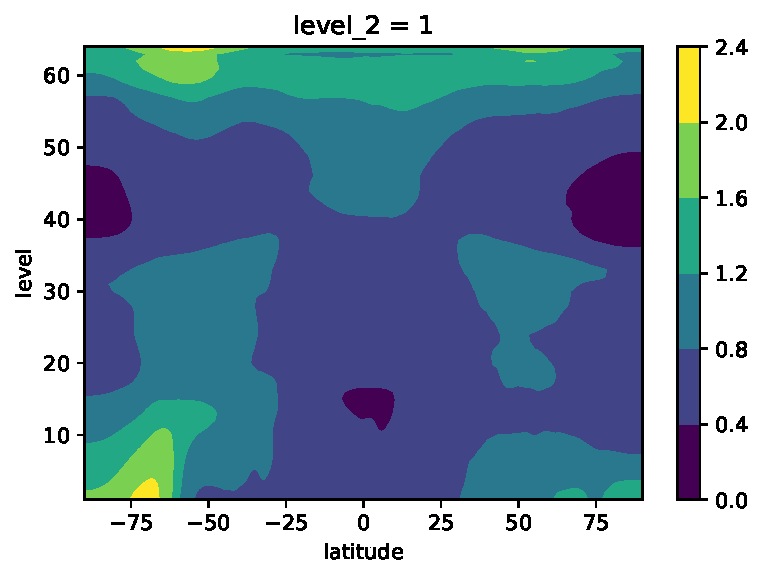
\includegraphics[width=0.25\textwidth]{./figs/Tv.pdf}};
%  \onslide<5-> \node[fill=white, align=right, text=black, font={\large\bfseries}] at (0,1.5) {$Tv$};
%  \onslide<4-> \node[inner sep=0pt] (image2) at (4,0) {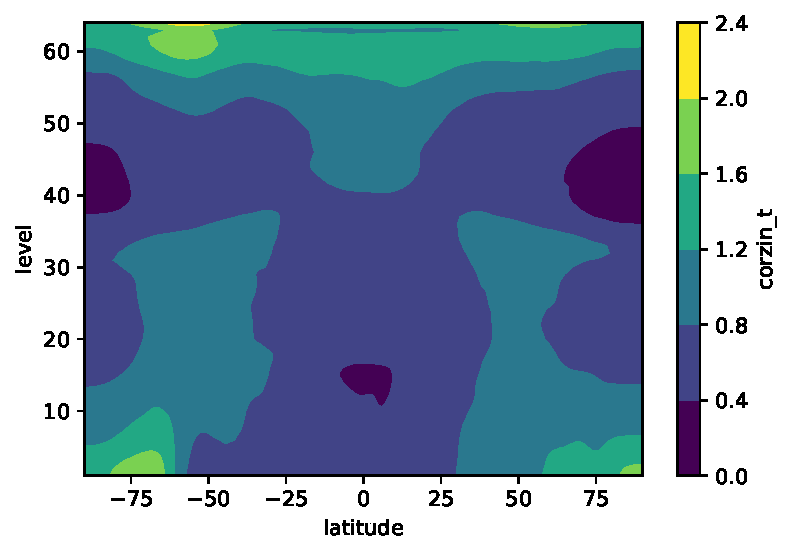
\includegraphics[width=0.25\textwidth]{./figs/Tv_u.pdf}};
%  \onslide<4-> \node[fill=white, align=right, text=black, font={\large\bfseries}] at (4,1.5) {$Tv_{u}$};
%  \onslide<2-> \node[inner sep=0pt] (image3) at (8,0) {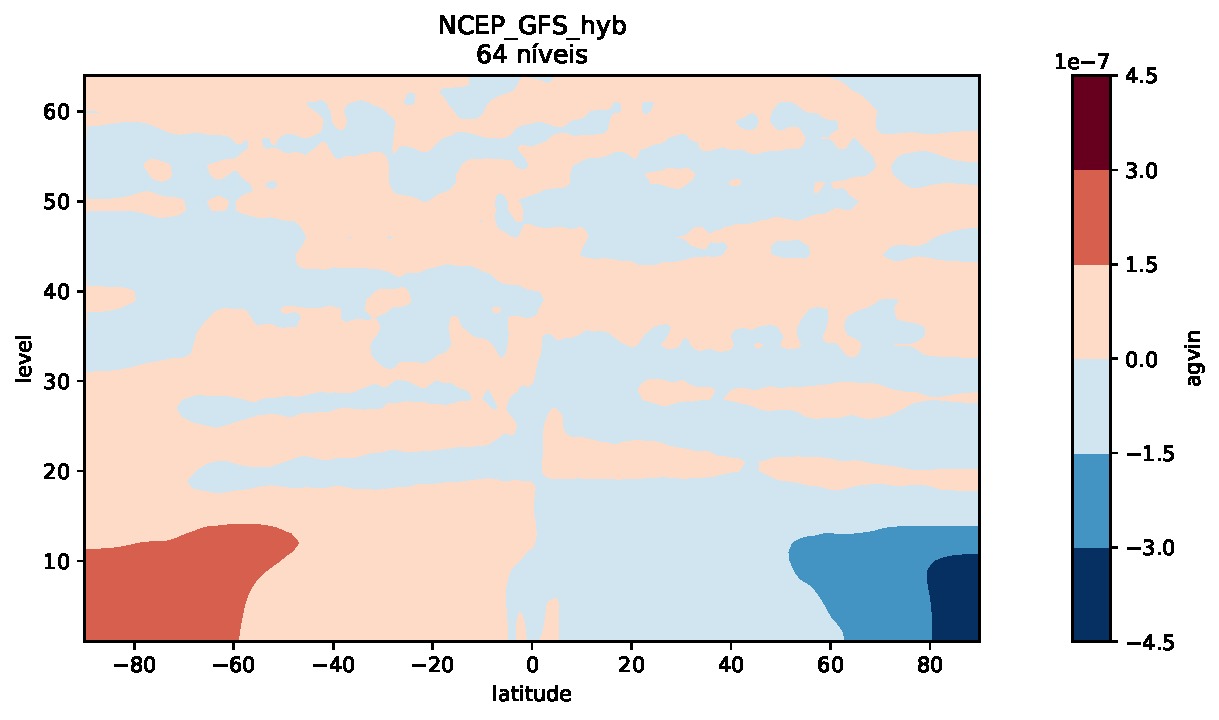
\includegraphics[width=0.25\textwidth]{./figs/agvin.pdf}};
%  \onslide<2-> \node[fill=white, align=right, text=black, font={\large\bfseries}] at (8,1.5) {$\mathbf{G}$};
%  \onslide<1-> \node[inner sep=0pt] (image4) at (12,0) {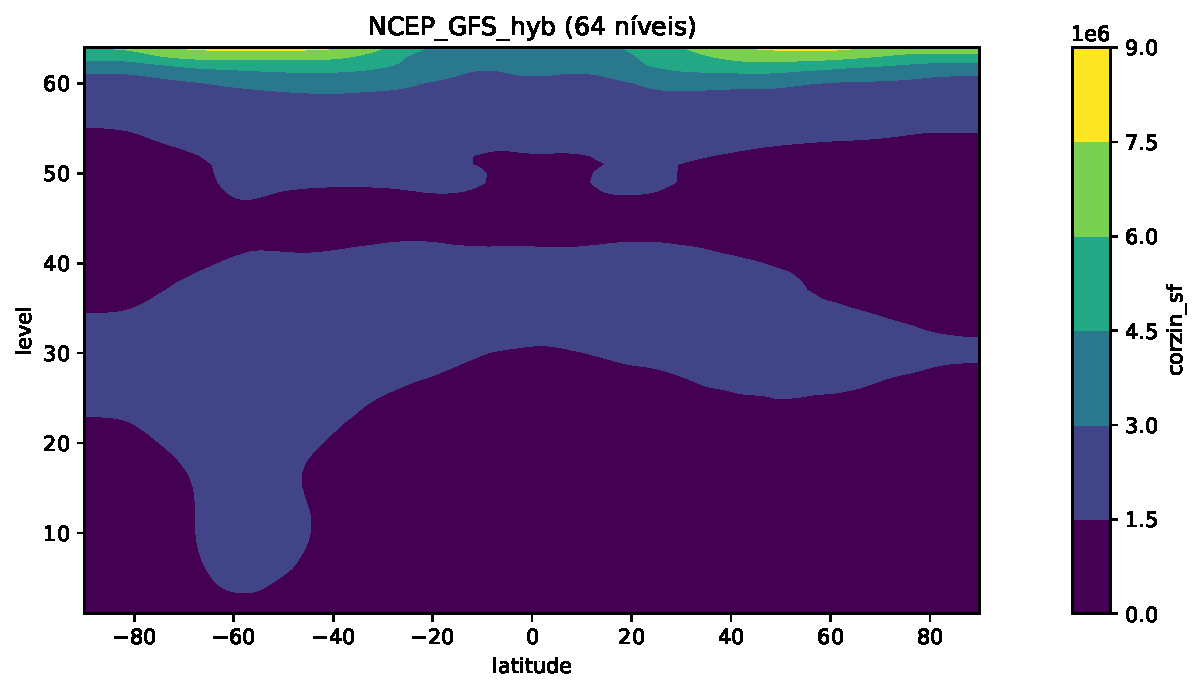
\includegraphics[width=0.25\textwidth]{./figs/sf.pdf}};
%  \node[fill=white, align=right, text=black, font={\large\bfseries}] at (12,1.5) {$\psi$};
%  \onslide<5-> \node[fill=white, align=right, text=black, font={\large\bfseries}] at (2,0) {$=$};
%  \onslide<4-> \node[fill=white, align=right, text=black, font={\large\bfseries}] at (6,0) {$+$};
%  \onslide<2-> \node[fill=white, align=right, text=black, font={\large\bfseries}] at (10,0) {$\times$};
%  
%  \onslide<3-> \draw [decorate] ([yshift=-10mm]image3.west) --node[below=3mm]{} ([yshift=-10mm]image4.east);
%
%  \onslide<5-> \node[inner sep=0pt] (image5) at (2,-3.1) {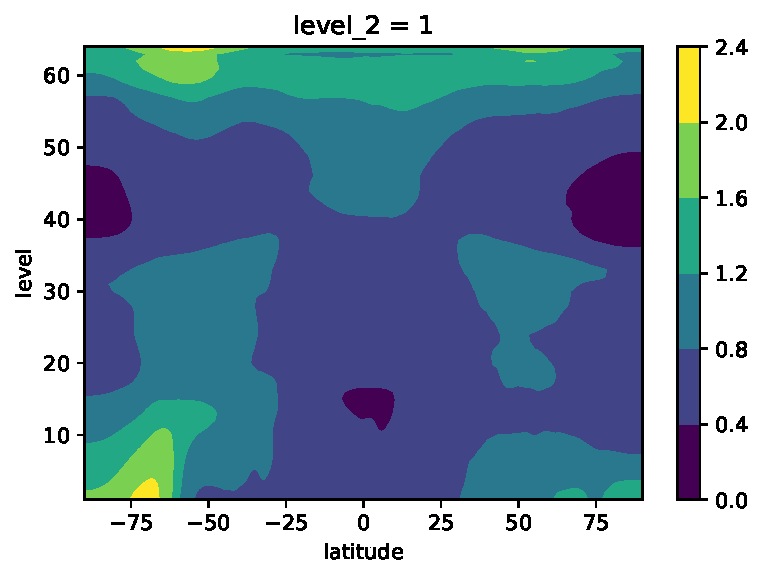
\includegraphics[width=0.25\textwidth]{./figs/Tv.pdf}};
%  \onslide<5-> \node[fill=white, align=right, text=black, font={\large\bfseries}] at (2,-1.6) {$Tv$};
%  \onslide<4-> \node[inner sep=0pt] (image6) at (6,-3.1) {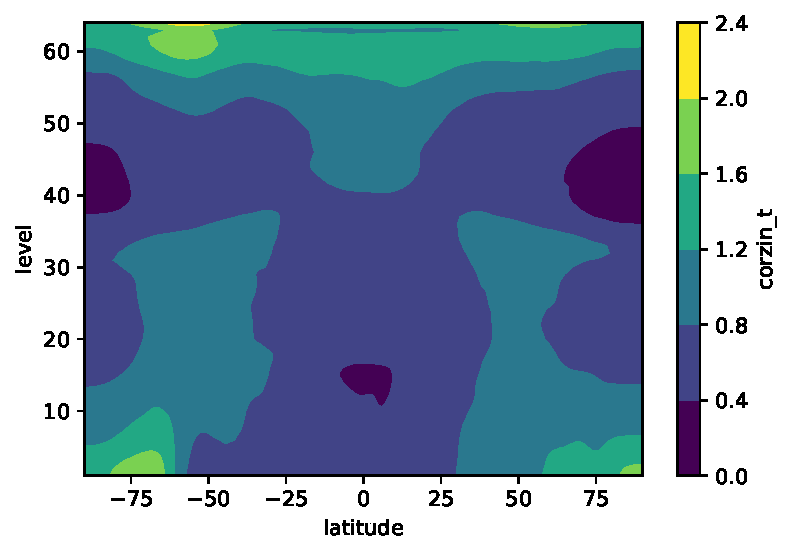
\includegraphics[width=0.25\textwidth]{./figs/Tv_u.pdf}};
%  \onslide<4-> \node[fill=white, align=right, text=black, font={\large\bfseries}] at (6,-1.6) {$Tv_{u}$};
%  \onslide<3-> \node[inner sep=0pt] (image7) at (10,-3.1) {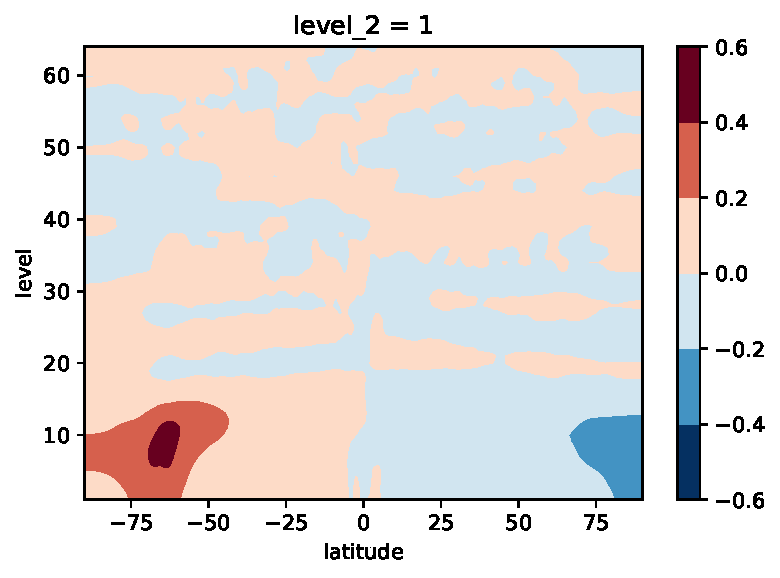
\includegraphics[width=0.25\textwidth]{./figs/Tv_b.pdf}};
%  \onslide<3-> \node[fill=white, align=right, text=black, font={\large\bfseries}] at (10,-1.6) {$\mathbf{G}\psi$};
%  \onslide<5-> \node[fill=white, align=right, text=black, font={\large\bfseries}] at (4,-3.1) {$=$};
%  \onslide<4-> \node[fill=white, align=right, text=black, font={\large\bfseries}] at (8,-3.1) {$+$};
%
%\end{tikzpicture}
%\end{block}
%\end{frame}

\begin{frame}[fragile]{Cálculo da Matriz $\mathbf{B}$}
\framesubtitle{Outros Aspectos}
\begin{block}{Contribuição de $\psi$ para $Tv$ ($Tv = Tv_{u} + \mathbf{G}\psi$):}
\hspace*{-2em}\begin{tikzpicture}[level/.style={},decoration={brace,mirror,amplitude=7}]

  \onslide<5-> \node[inner sep=0pt] (image1) at (0,0) {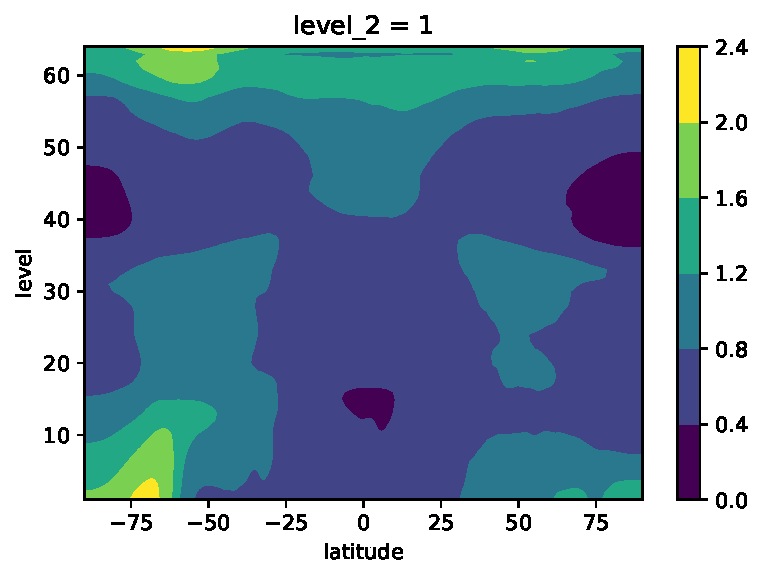
\includegraphics[width=0.25\textwidth]{./figs/Tv.pdf}};
  \onslide<5-> \node[fill=white, align=right, text=black, font={\large\bfseries}] at (0,1.5) {$Tv$};
  \onslide<4-> \node[inner sep=0pt] (image2) at (4,0) {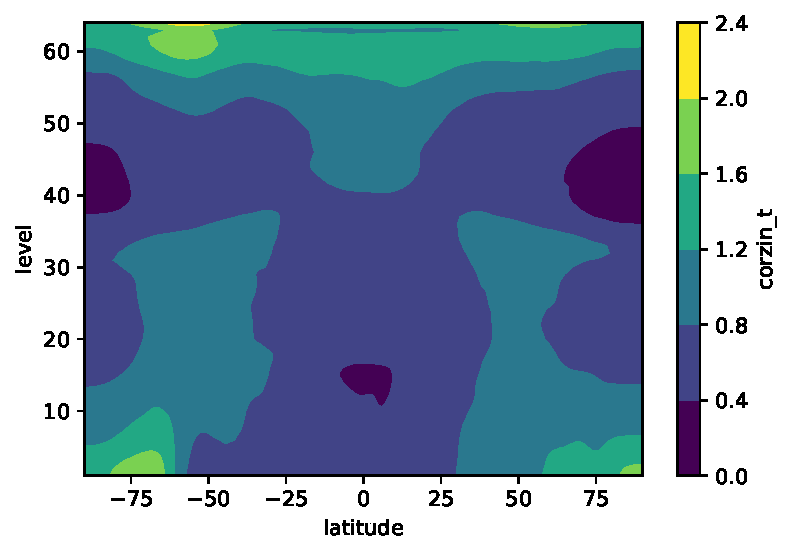
\includegraphics[width=0.25\textwidth]{./figs/Tv_u.pdf}};
  \onslide<4-> \node[fill=white, align=right, text=black, font={\large\bfseries}] at (4,1.5) {$Tv_{u}$};
  \onslide<2-> \node[inner sep=0pt] (image3) at (8,0) {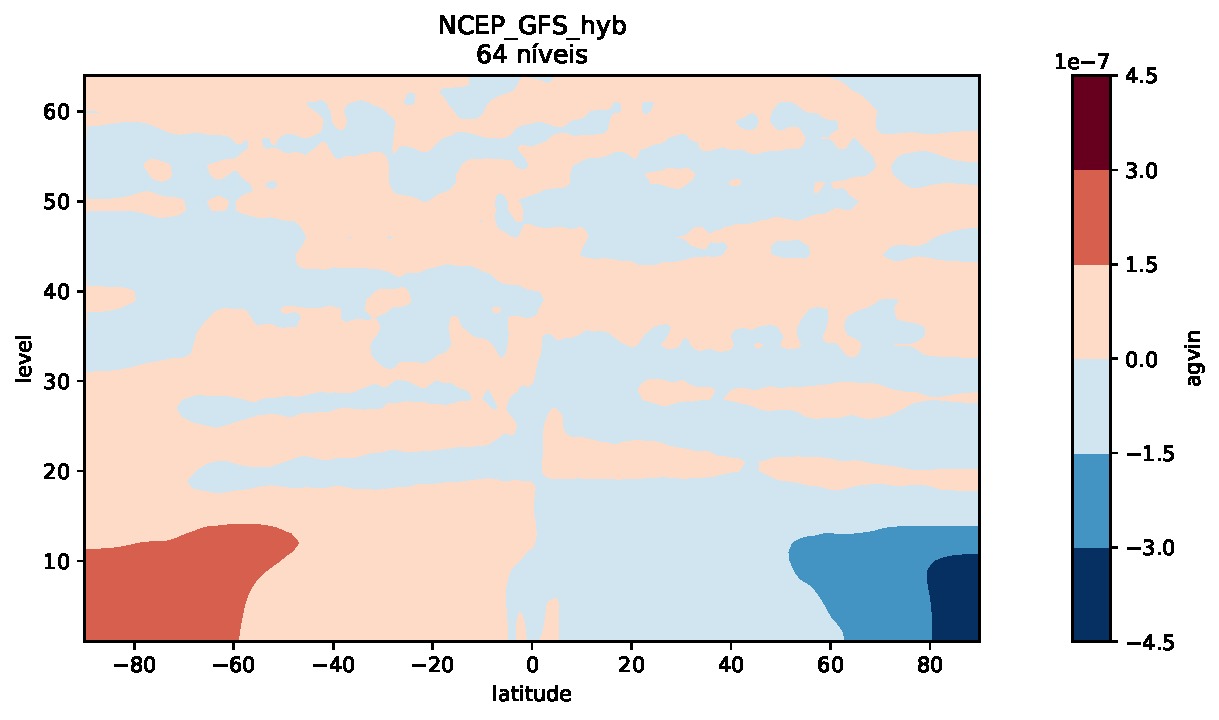
\includegraphics[width=0.25\textwidth]{./figs/agvin.pdf}};
  \onslide<2-> \node[fill=white, align=right, text=black, font={\large\bfseries}] at (8,1.5) {$\mathbf{G}$};
  \onslide<1-> \node[inner sep=0pt] (image4) at (12,0) {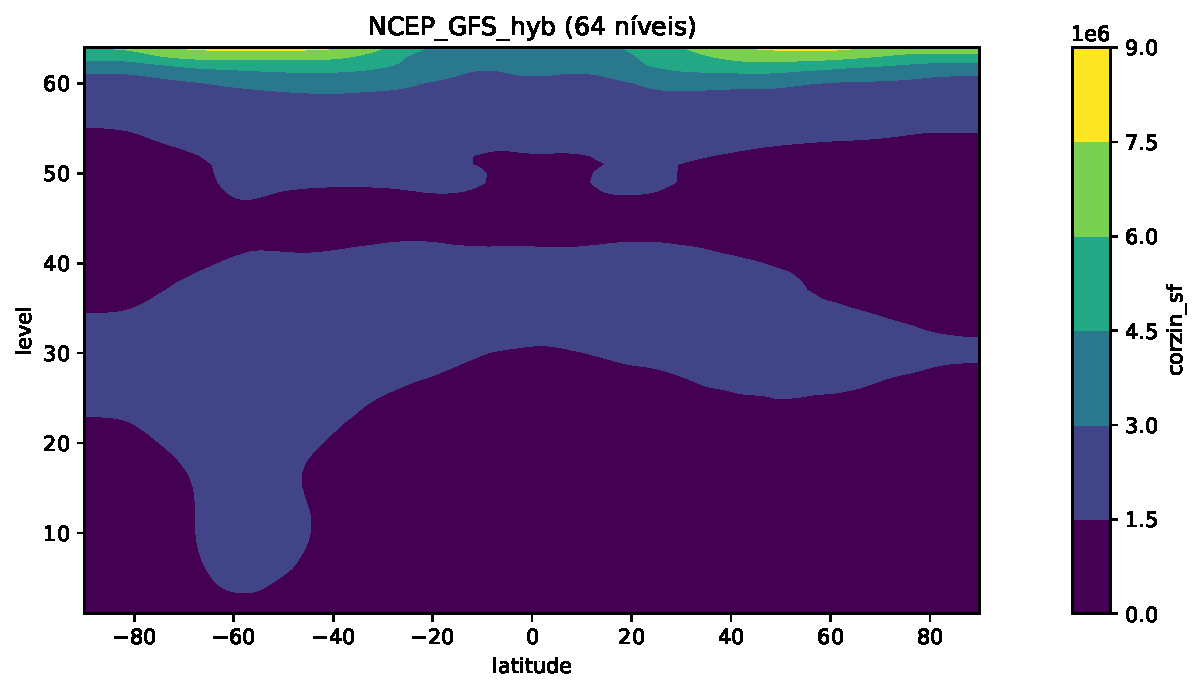
\includegraphics[width=0.25\textwidth]{./figs/sf.pdf}};
  \node[fill=white, align=right, text=black, font={\large\bfseries}] at (12,1.5) {$\psi$};
  \onslide<5-> \node[fill=white, align=right, text=black, font={\large\bfseries}] at (2,0) {$=$};
  \onslide<4-> \node[fill=white, align=right, text=black, font={\large\bfseries}] at (6,0) {$+$};
  \onslide<2-> \node[fill=white, align=right, text=black, font={\large\bfseries}] at (10,0) {$\times$};
  
  \onslide<3-> \draw [decorate] ([yshift=-10mm]image3.west) --node[below=3mm]{} ([yshift=-10mm]image4.east);

  \onslide<5-> \node[inner sep=0pt] (image5) at (2,-3.1) {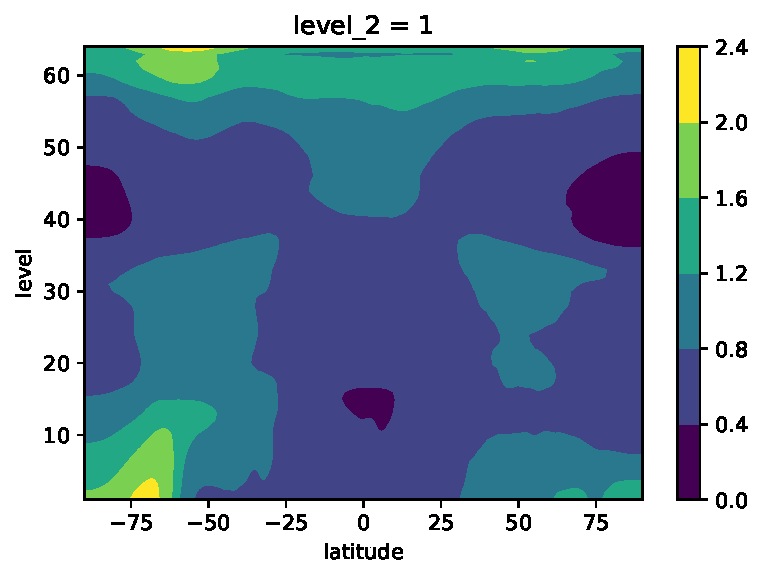
\includegraphics[width=0.25\textwidth]{./figs/Tv.pdf}};
  \onslide<5-> \node[fill=white, align=right, text=black, font={\large\bfseries}] at (2,-1.6) {$Tv$};
  \onslide<4-> \node[inner sep=0pt] (image6) at (6,-3.1) {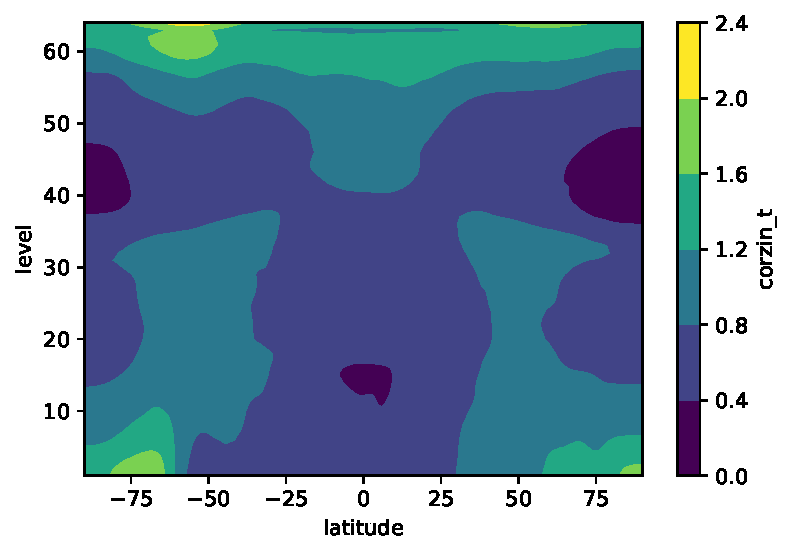
\includegraphics[width=0.25\textwidth]{./figs/Tv_u.pdf}};
  \onslide<4-> \node[fill=white, align=right, text=black, font={\large\bfseries}] at (6,-1.6) {$Tv_{u}$};
  \onslide<3-> \node[inner sep=0pt] (image7) at (10,-3.1) {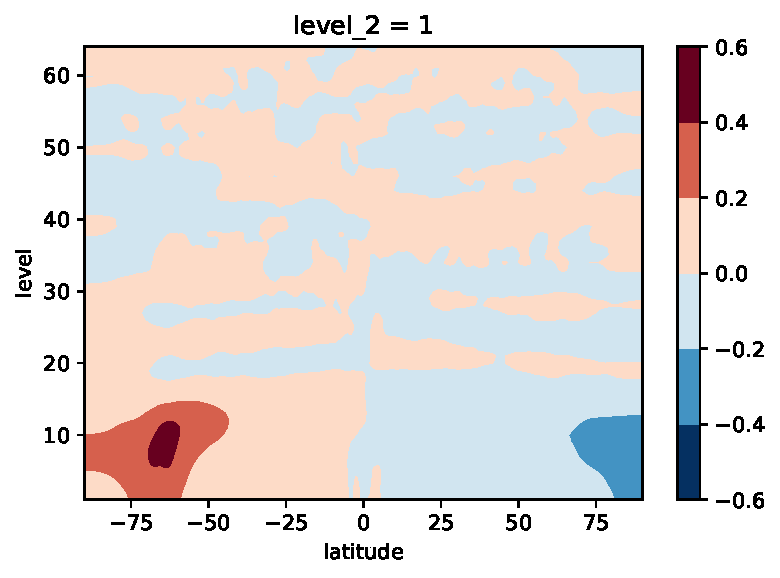
\includegraphics[width=0.25\textwidth]{./figs/Tv_b.pdf}};
  \onslide<3-> \node[fill=white, align=right, text=black, font={\large\bfseries}] at (10,-1.6) {$\mathbf{G}\psi$};
  \onslide<5-> \node[fill=white, align=right, text=black, font={\large\bfseries}] at (4,-3.1) {$=$};
  \onslide<4-> \node[fill=white, align=right, text=black, font={\large\bfseries}] at (8,-3.1) {$+$};

\end{tikzpicture}
\end{block}
\end{frame}

\section{Resultados}

\subsection{Produção Técnica}

\begin{frame}{Resultados}
\framesubtitle{Produção Técnica~\faCogs}
    \begin{itemize}
        \item \faIcon[regular]{file}~Artigo com a aplicação deste método NMC baseado no modelo BAM V0 \cite{figueroaetal/2016}: \textbf{``Matriz de Covariâncias dos Erros de Previsão Aplicada ao Sistema de Assimilação de Dados Global do CPTEC: Experimentos com Observação Única''} \cite{bastarz/2017};
        \pause
        \item \faCode~Técnica para o cálculo da matriz $\mathbf{B}$ baseada no programa escrito pelo \href{https://community.wmo.int/contacts/dr-daryl-t-kleist}{Dr. Daryl Kleist} (\href{https://www.weather.gov/ncep/}{NCEP}) - podemos recalcular a matriz sempre que o modelo sofrer alterações;
        \pause
        \item \faCode~\href{https://github.com/GAD-DIMNT-CPTEC/GSIBerror}{GSIBerror}: pacote Python para a leitura, plotagem e comparação de matrizes de covariâncias compatíveis com o GSI no formato \texttt{.gcv} \cite{bastarz/2022};
        \pause
        \begin{itemize}
        	\item \faPython~Demonstração disponível: \href{https://mybinder.org/v2/gh/cfbastarz/GSIBerror/main}{
\includegraphics[width=1.5cm]{binder.png}}
        \end{itemize}
        \pause
        \item \faFlask~Preparação de uma matriz baseada no BAM V2.1.0 (em coordenada híbrida) para uso com o GSI na assimilação de dados (exemplo nos próximos slides).
    \end{itemize}
\end{frame}

%\subsection{Matrizes de Projeção}
%
%\begin{frame}{Resultados}
%\framesubtitle{Matrizes de Projeção}
%\begin{figure}[H]
%    \begin{center}
%        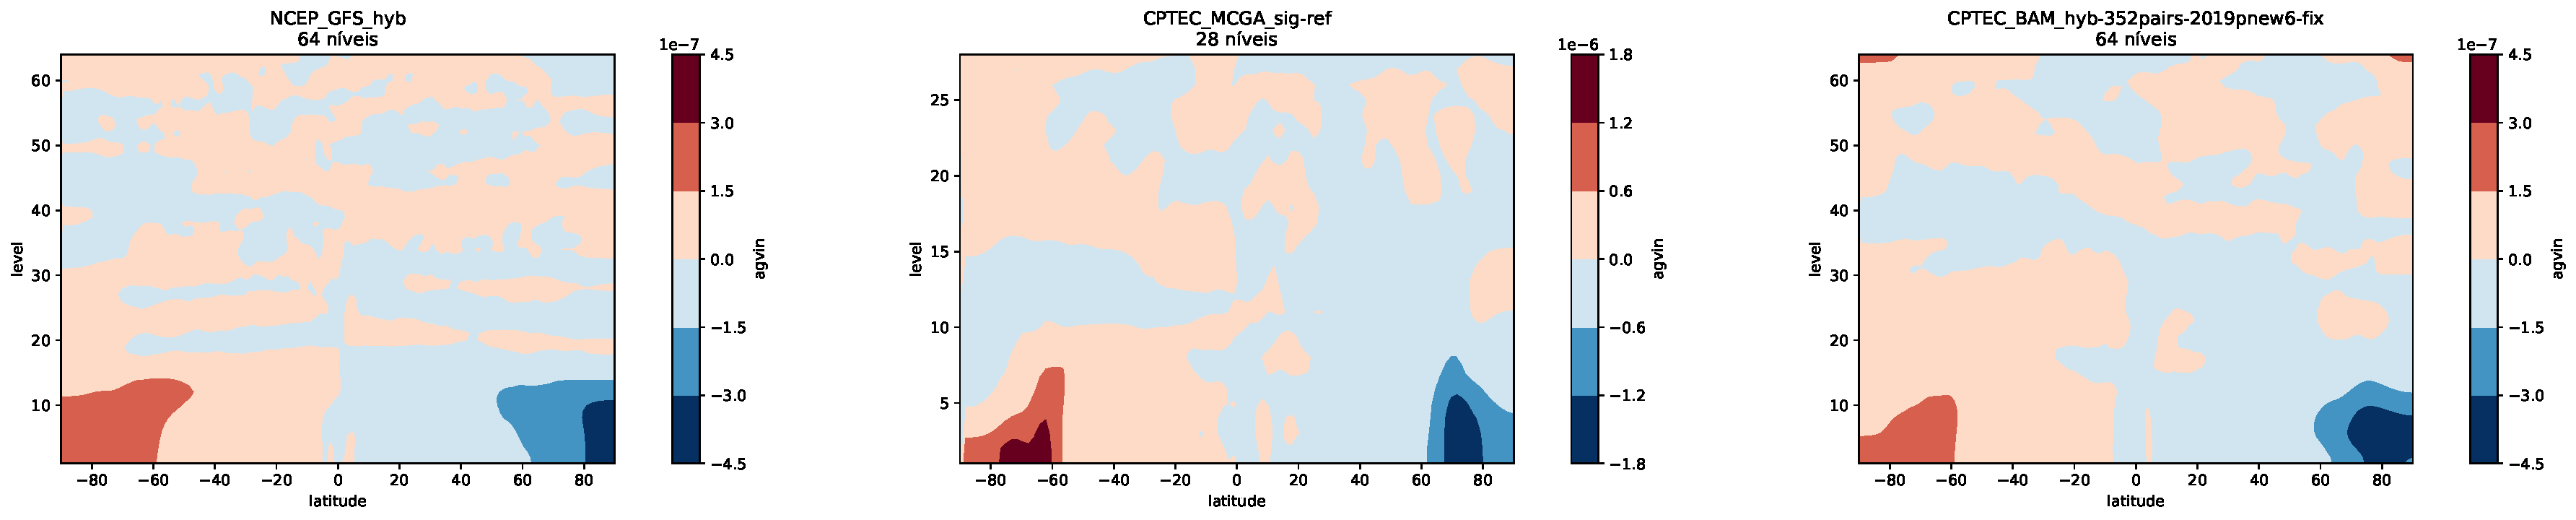
\includegraphics[width=1.\textwidth]{./figs/compara/agvin.pdf}
%        \caption{Projeção da $\psi$ no nível 0 sobre o perfil da parte balanceada da $Tv$ ($Tb = \mathbf{G}\psi$).}
%    \end{center}
%\end{figure}
%\end{frame}
%
%\begin{frame}{Resultados}
%\framesubtitle{Matrizes de Projeção}
%\begin{figure}[H]
%    \begin{center}
%        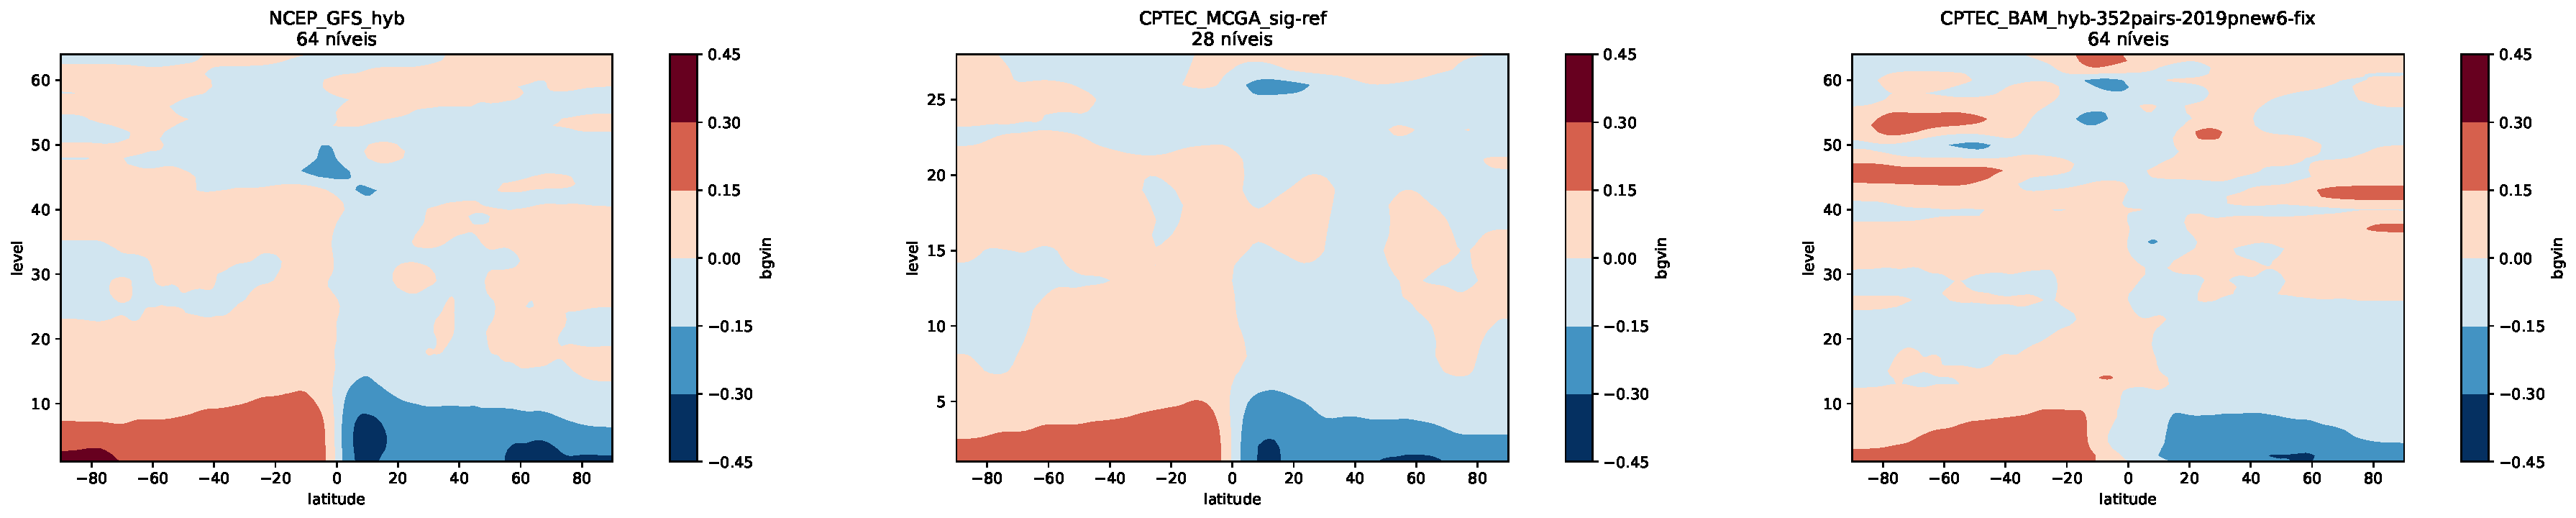
\includegraphics[width=1.\textwidth]{./figs/compara/bgvin.pdf}
%        \caption{Projeção da $\psi$ no nível 0 sobre o perfil da parte balanceada de $\chi$ ($\chi_{b} = \mathbf{c}\psi$).}
%    \end{center}
%\end{figure}
%\end{frame}
%
%\begin{frame}{Resultados}
%\framesubtitle{Matrizes de Projeção}
%\begin{figure}[H]
%    \begin{center}
%        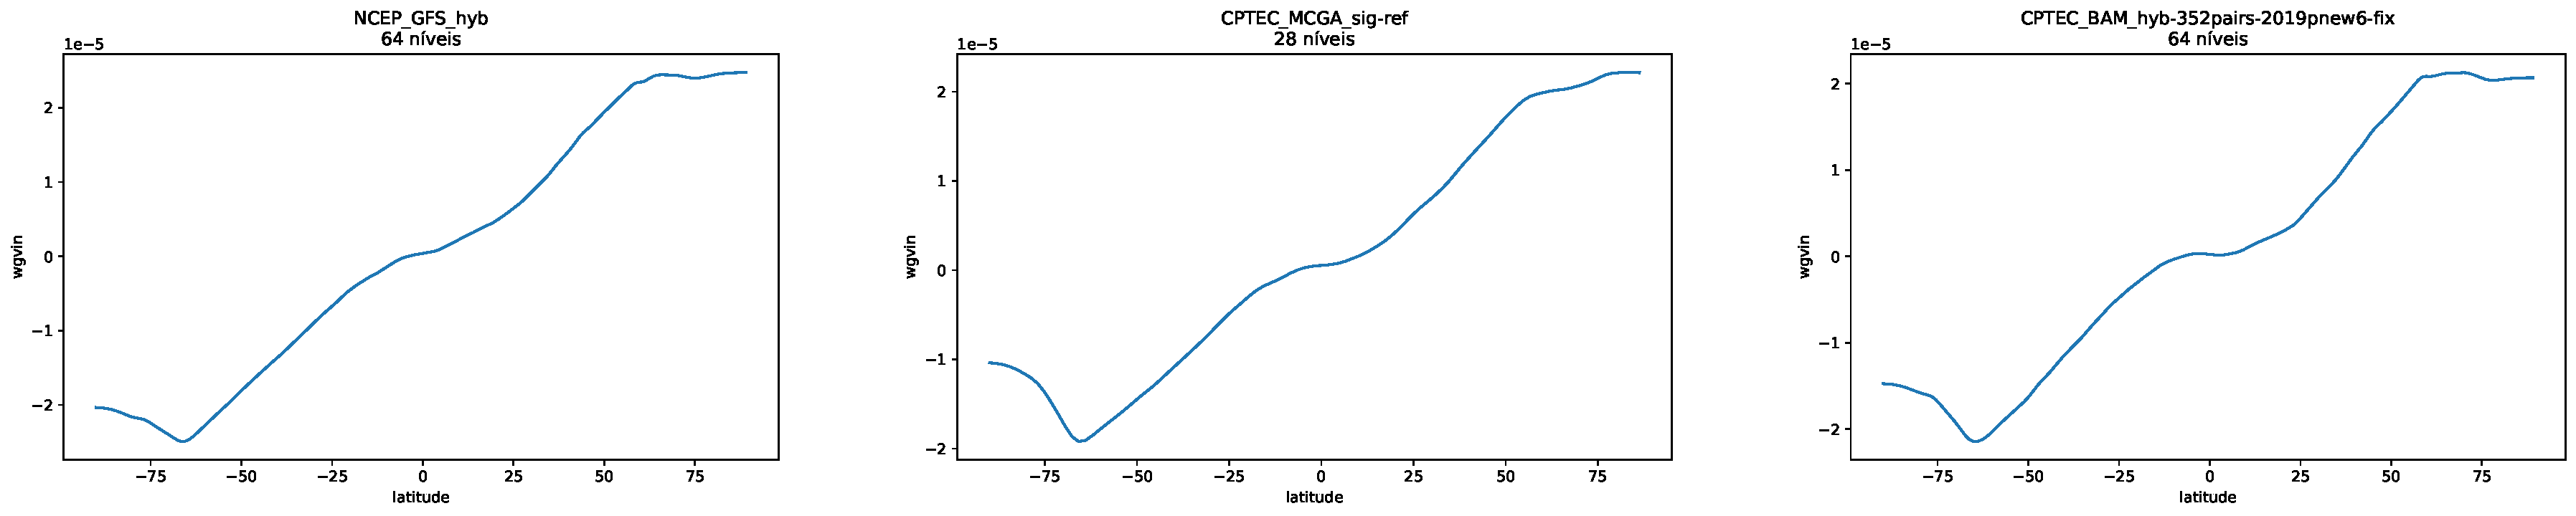
\includegraphics[width=1.\textwidth]{./figs/compara/wgvin.pdf}
%        \caption{Projeção da $\psi$ sobre a parte balanceada da $ps$ ($ps_{b} = \mathbf{w}\psi$).}
%    \end{center}
%\end{figure}
%\end{frame}

%\subsection{Desvios-padrão}
%
%%\begin{frame}{Resultados}
%%\framesubtitle{Desvios-padrão}
%%\begin{figure}[H]
%%    \begin{center}
%%        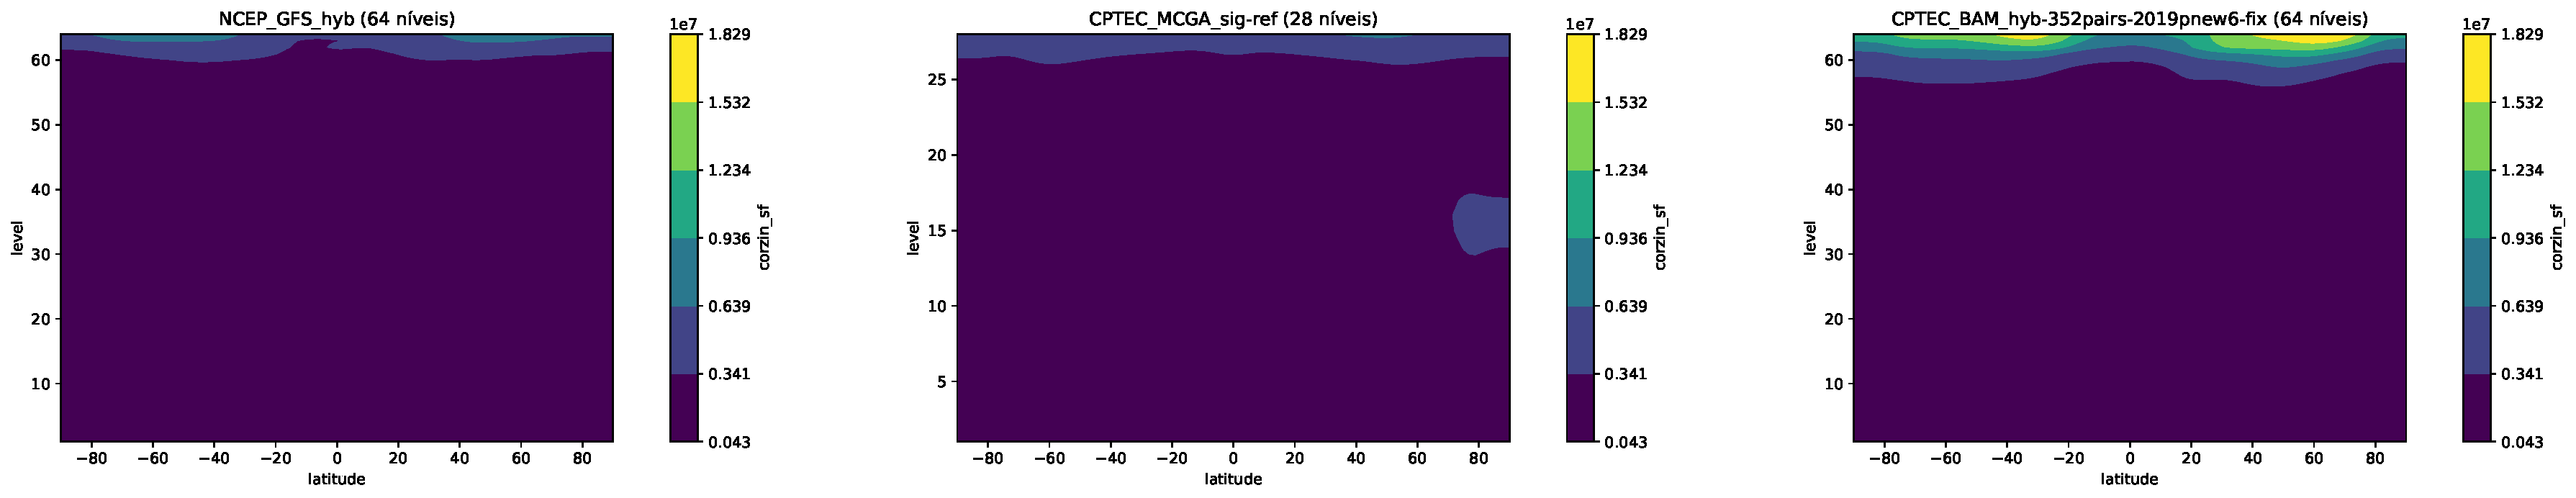
\includegraphics[width=1.\textwidth]{./figs/compara/sf.pdf}
%%        \caption{Desvio-padrão da $\psi$.}
%%    \end{center}
%%\end{figure}
%%\end{frame}
%%
%%\begin{frame}{Resultados}
%%\framesubtitle{Desvios-padrão}
%%\begin{figure}[H]
%%    \begin{center}
%%        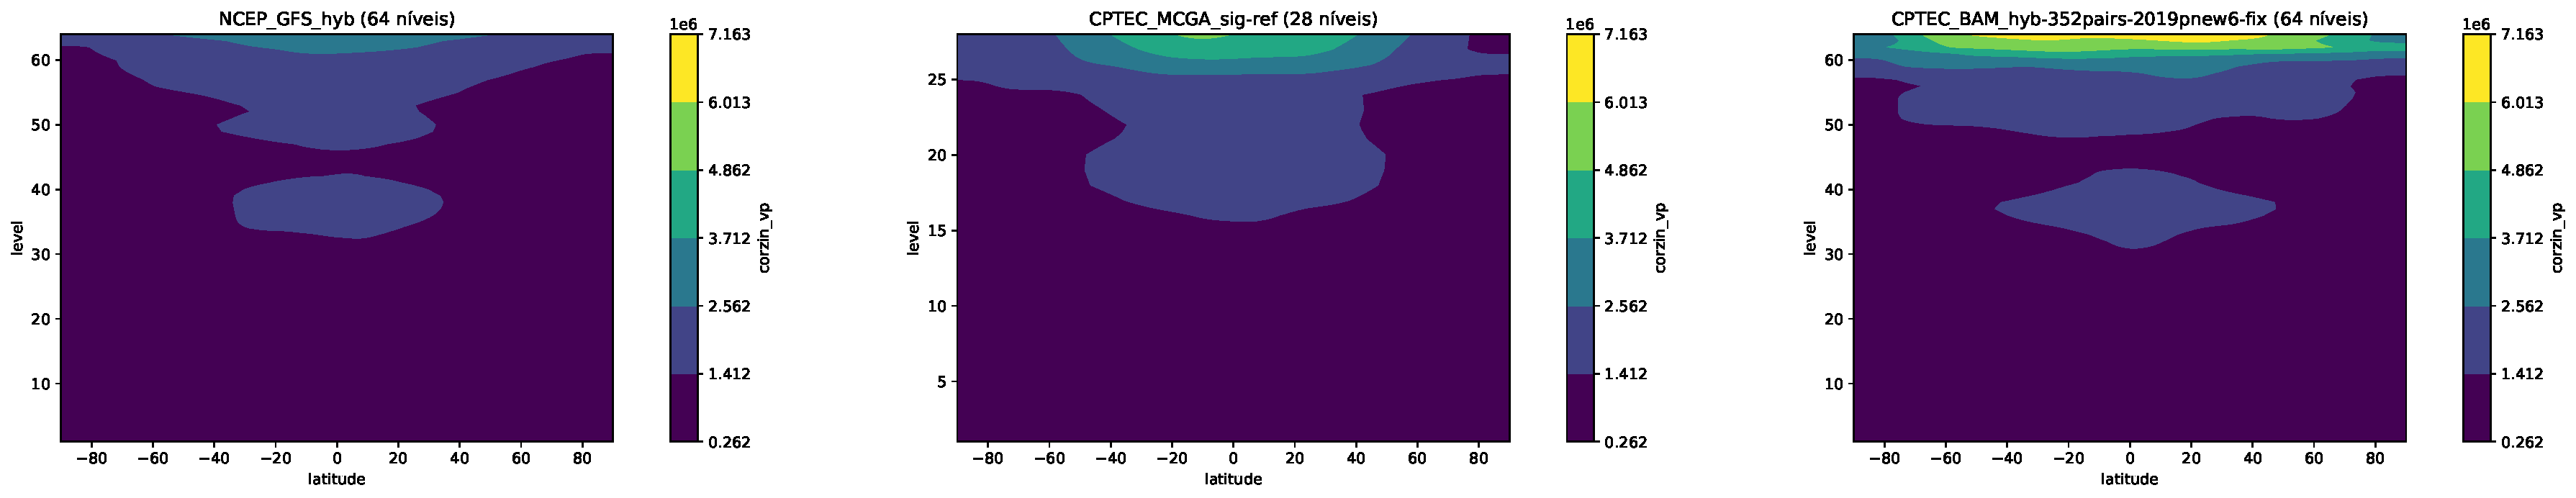
\includegraphics[width=1.\textwidth]{./figs/compara/vp.pdf}
%%        \caption{Desvio-padrão da $\chi$.}
%%    \end{center}
%%\end{figure}
%%\end{frame}
%
%\begin{frame}{Resultados}
%\framesubtitle{Desvios-padrão}
%\begin{figure}[H]
%    \begin{center}
%        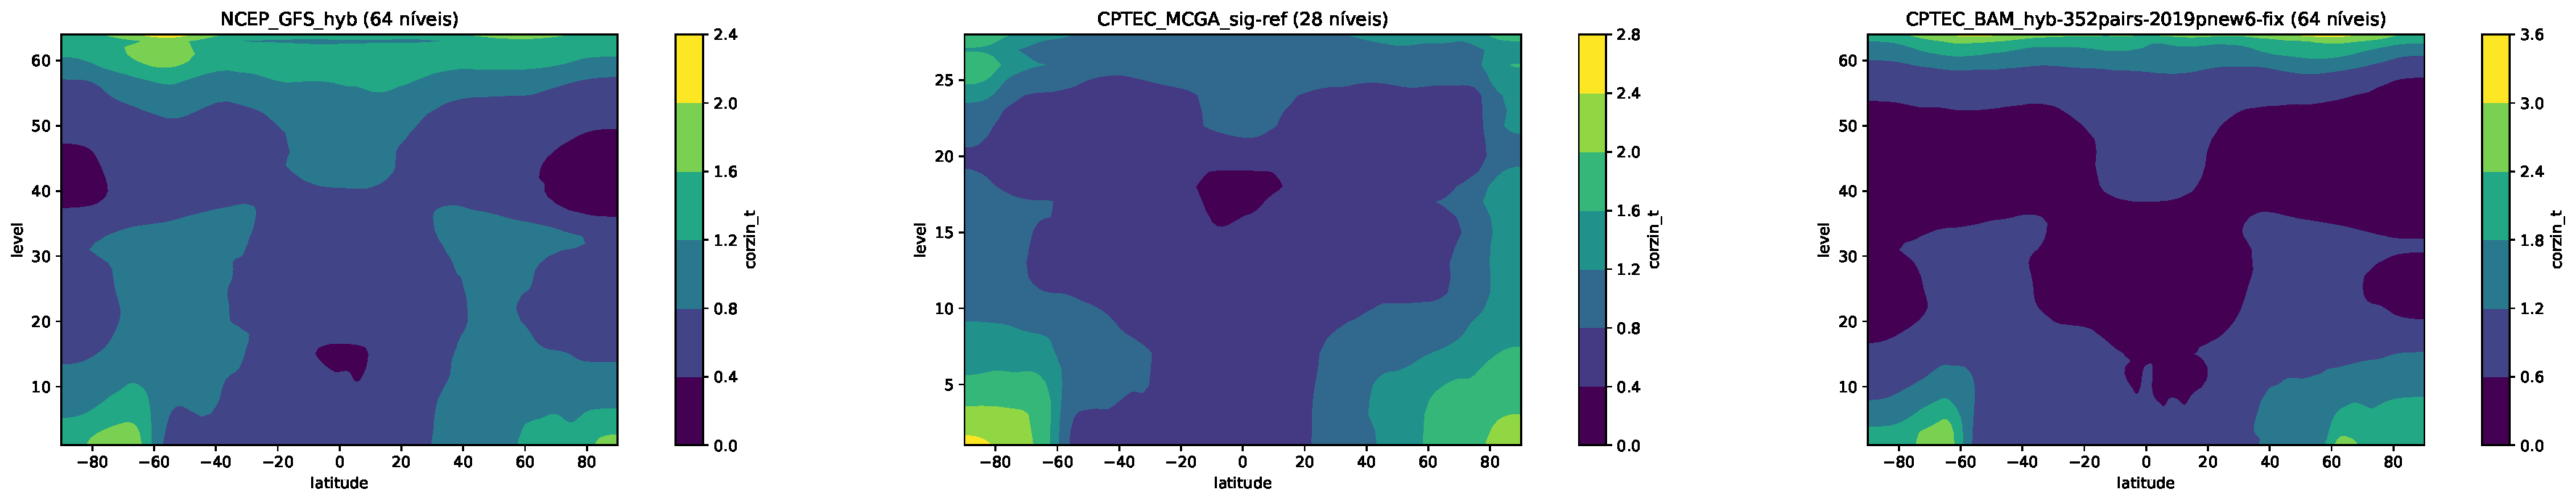
\includegraphics[width=1.\textwidth]{./figs/compara/t.pdf}
%        \caption{Desvio-padrão da $Tv$.}
%    \end{center}
%\end{figure}
%\end{frame}
%
%%\begin{frame}{Resultados}
%%\framesubtitle{Desvios-padrão}
%%\begin{figure}[H]
%%    \begin{center}
%%        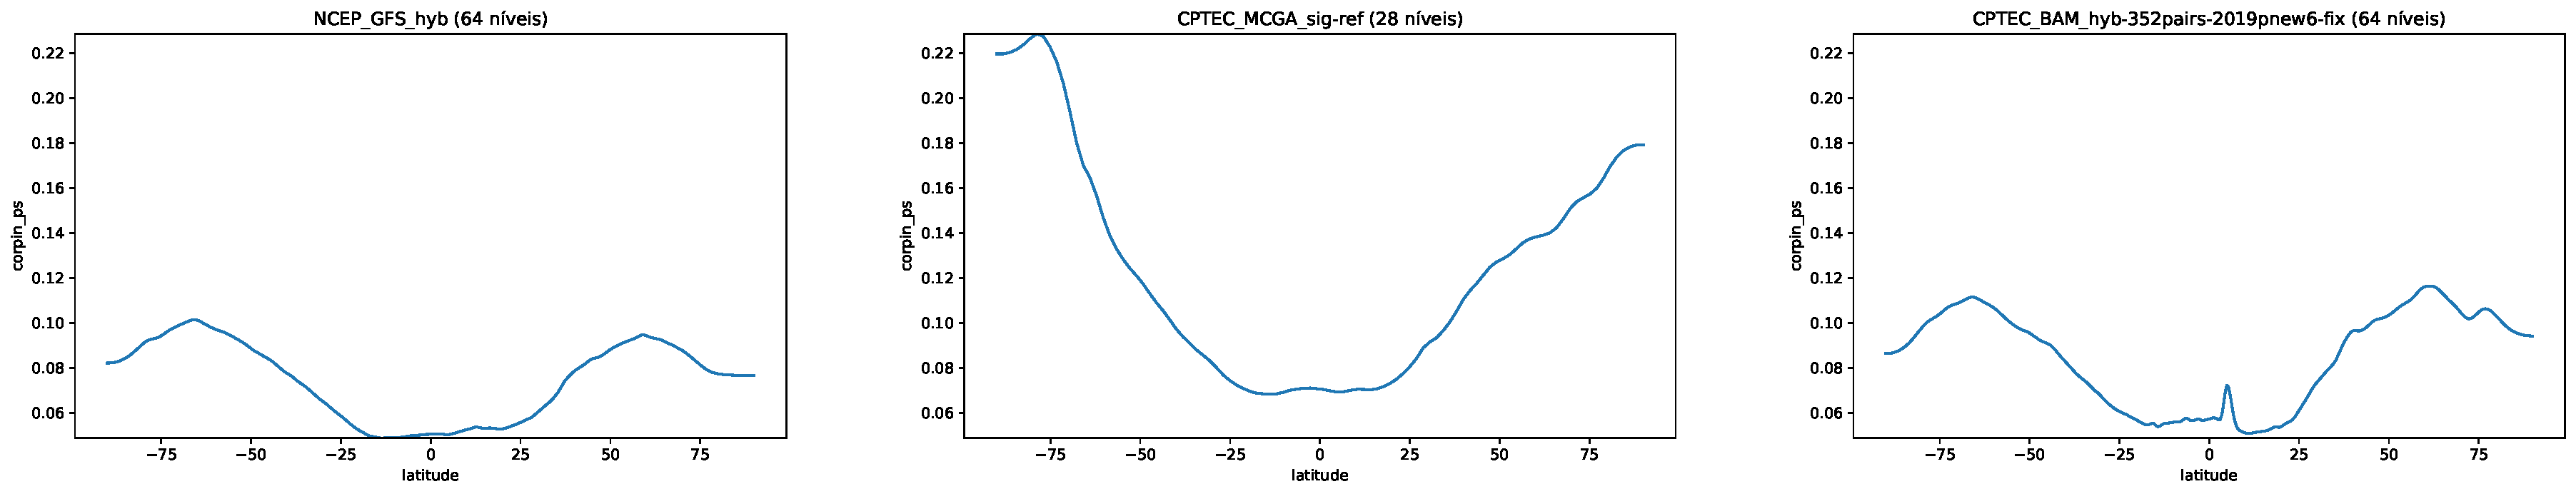
\includegraphics[width=1.\textwidth]{./figs/compara/ps.pdf}
%%        \caption{Desvio-padrão da $ps$.}
%%    \end{center}
%%\end{figure}
%%\end{frame}
%
%\subsection{Comprimentos de Escala (Horiz./Vert.)}
%
%%\begin{frame}{Resultados}
%%\framesubtitle{Comprimentos de Escala (Horizontais)}
%%\begin{figure}[H]
%%    \begin{center}
%%        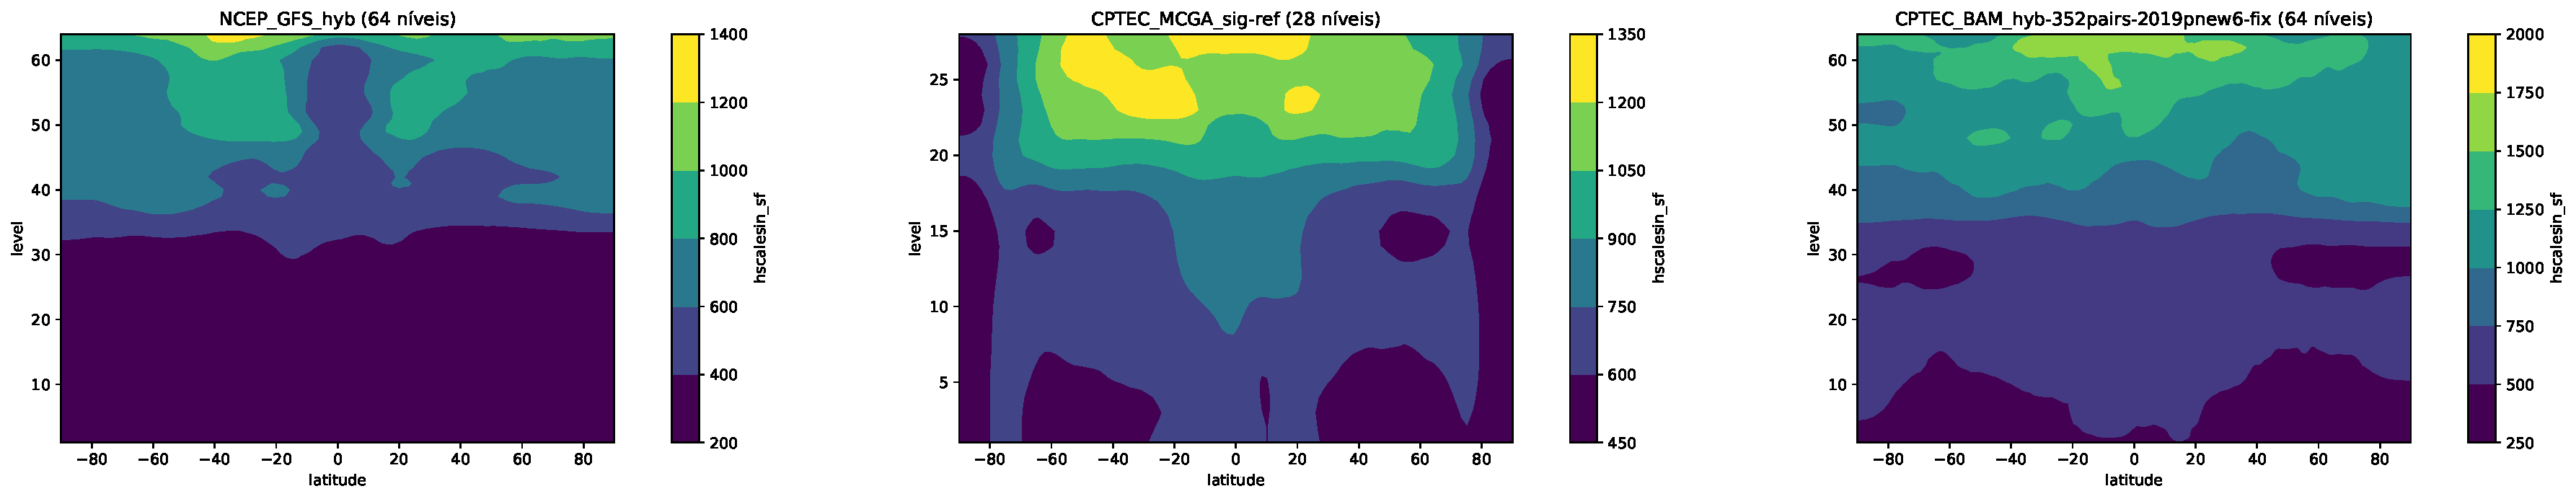
\includegraphics[width=1.\textwidth]{./figs/compara/hs_sf.pdf}
%%        \caption{Comprimento de Escala Horizontal da $\psi$.}
%%    \end{center}
%%\end{figure}
%%\end{frame}
%%
%%\begin{frame}{Resultados}
%%\framesubtitle{Comprimentos de Escala (Horizontais)}
%%\begin{figure}[H]
%%    \begin{center}
%%        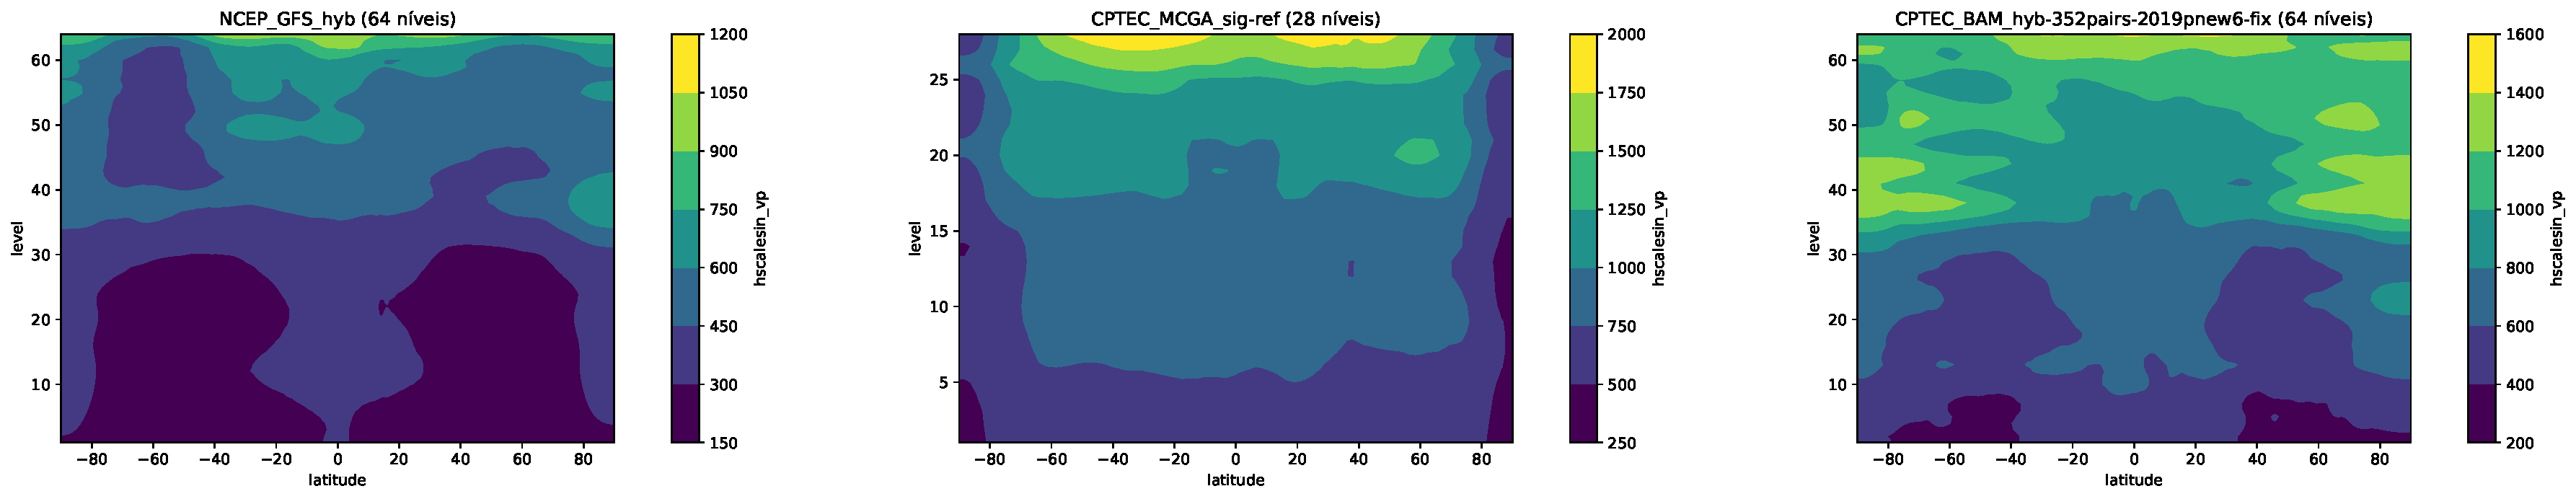
\includegraphics[width=1.\textwidth]{./figs/compara/hs_vp.pdf}
%%        \caption{Comprimento de Escala Horizontal da $\chi$.}
%%    \end{center}
%%\end{figure}
%%\end{frame}
%
%\begin{frame}{Resultados}
%\framesubtitle{Comprimentos de Escala (Horizontais)}
%\begin{figure}[H]
%    \begin{center}
%        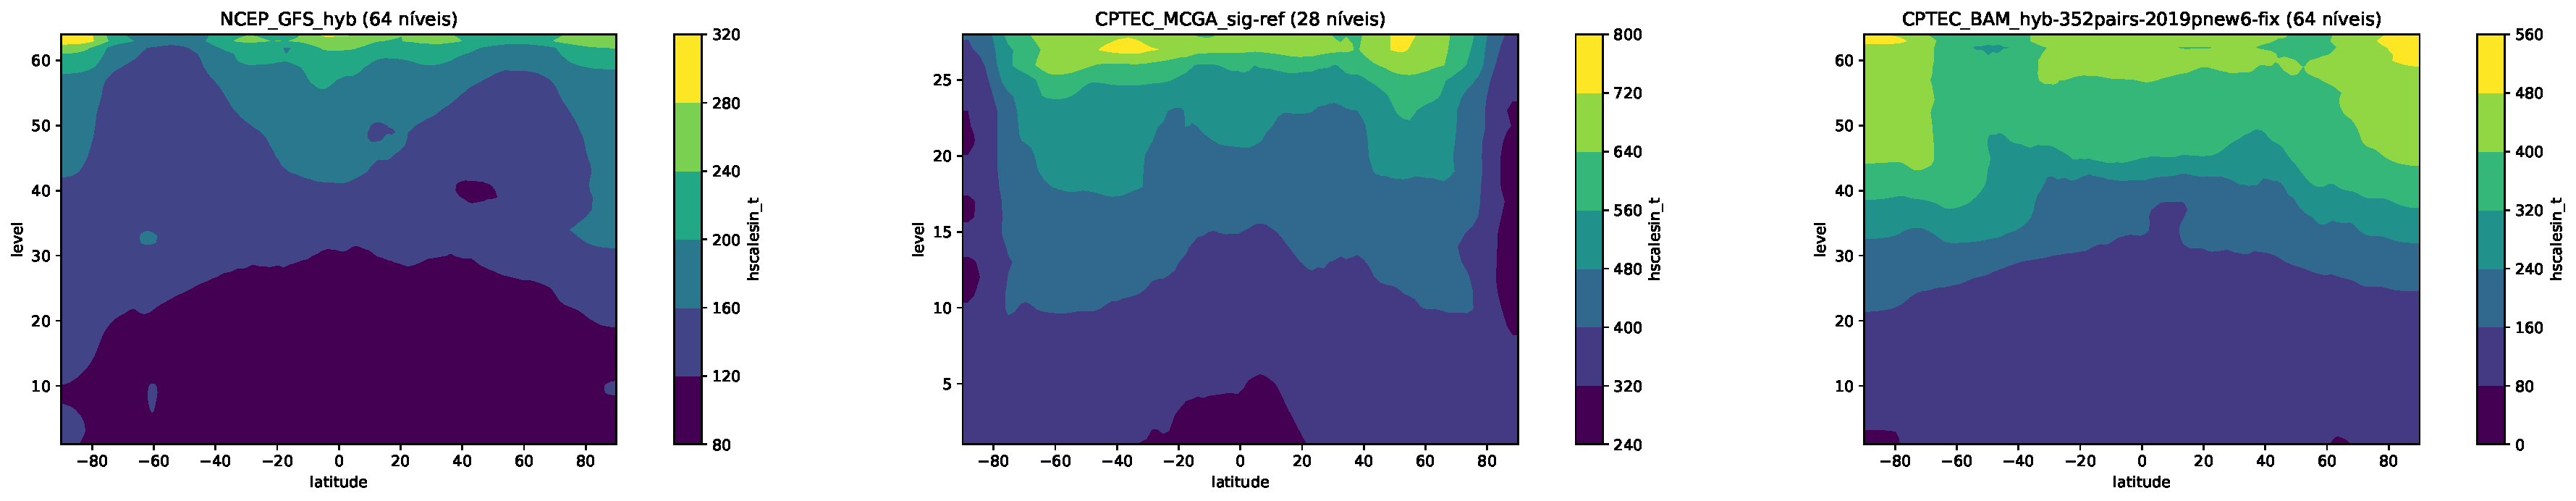
\includegraphics[width=1.\textwidth]{./figs/compara/hs_t.pdf}
%        \caption{Comprimento de Escala Horizontal da $Tv$.}
%    \end{center}
%\end{figure}
%\end{frame}
%
%%\begin{frame}{Resultados}
%%\framesubtitle{Comprimentos de Escala (Horizontais)}
%%\begin{figure}[H]
%%    \begin{center}
%%        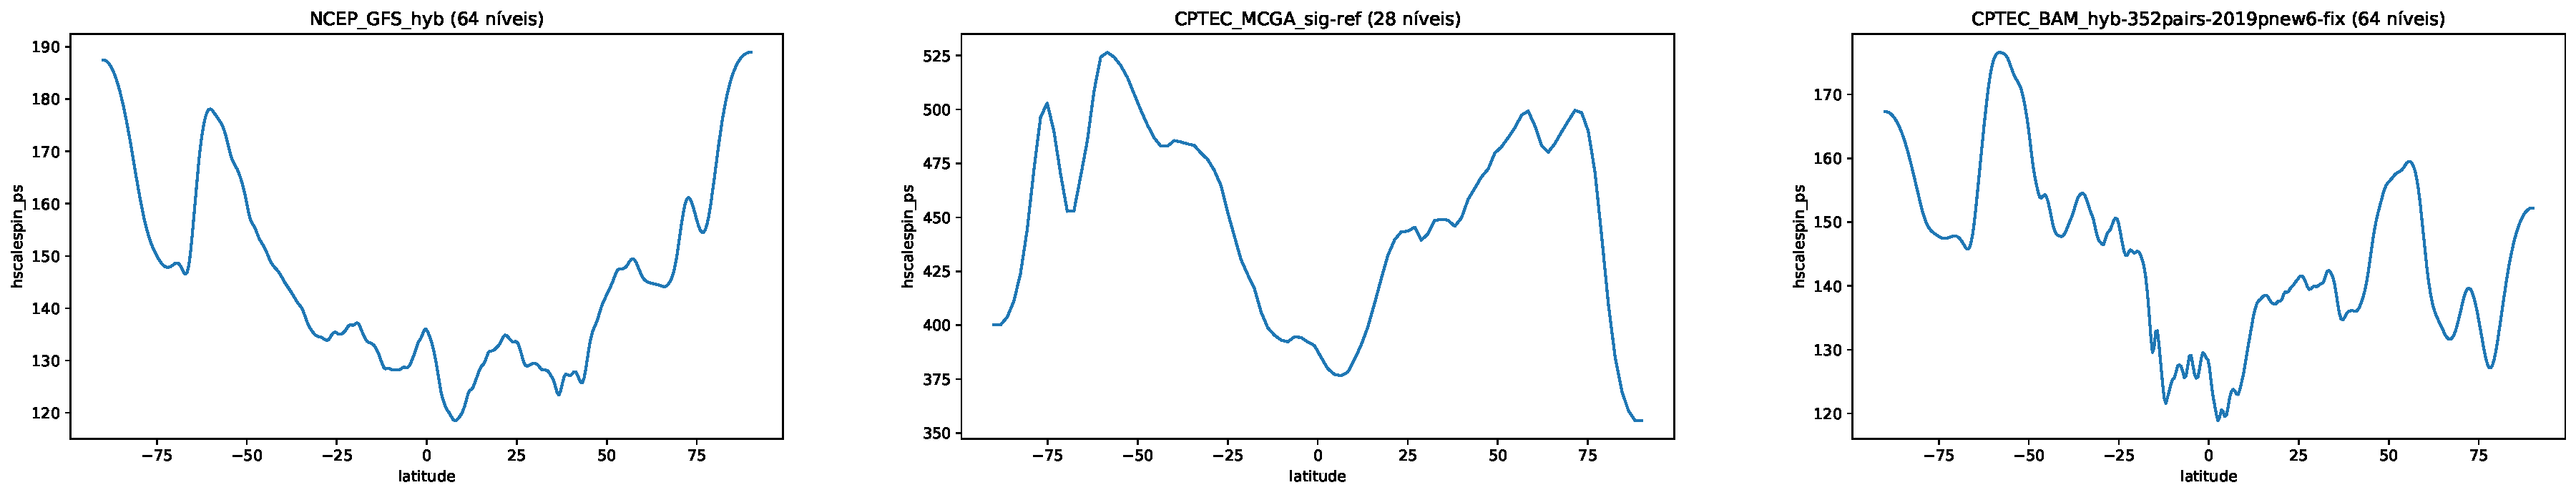
\includegraphics[width=1.\textwidth]{./figs/compara/hs_ps.pdf}
%%        \caption{Comprimento de Escala Horizontal da $ps$.}
%%    \end{center}
%%\end{figure}
%%\end{frame}
%
%%\begin{frame}{Resultados}
%%\framesubtitle{Comprimentos de Escala (Verticais)}
%%\begin{figure}[H]
%%    \begin{center}
%%        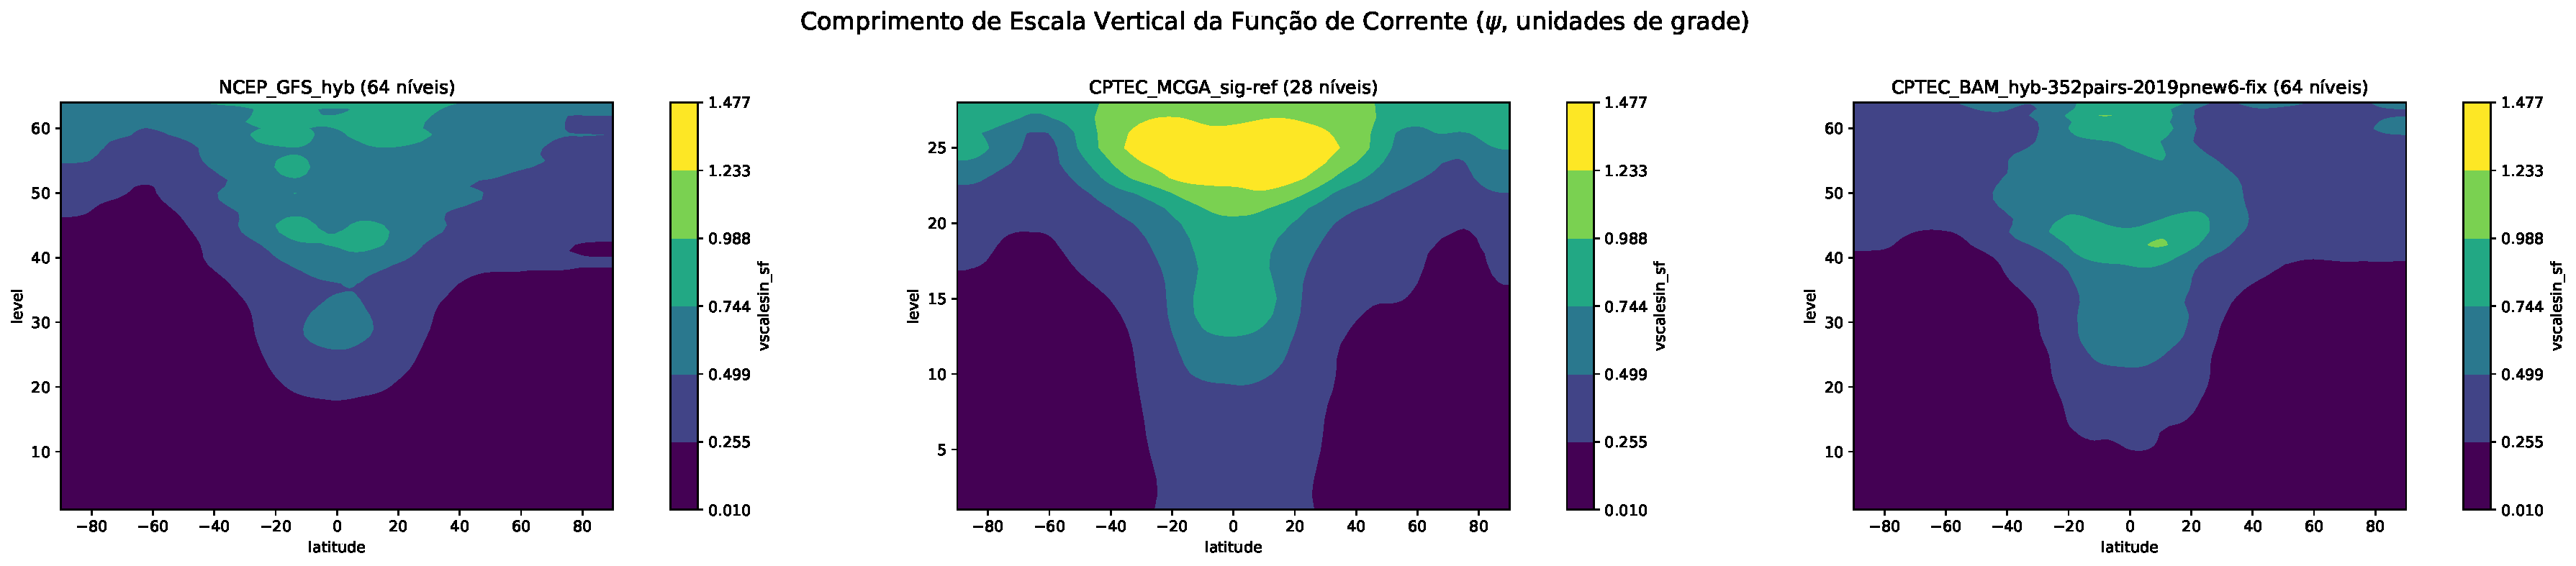
\includegraphics[width=1.\textwidth]{./figs/compara/vs_sf.pdf}
%%        \caption{Comprimento de Escala Vertical da $\psi$.}
%%    \end{center}
%%\end{figure}
%%\end{frame}
%%
%%\begin{frame}{Resultados}
%%\framesubtitle{Comprimentos de Escala (Verticais)}
%%\begin{figure}[H]
%%    \begin{center}
%%        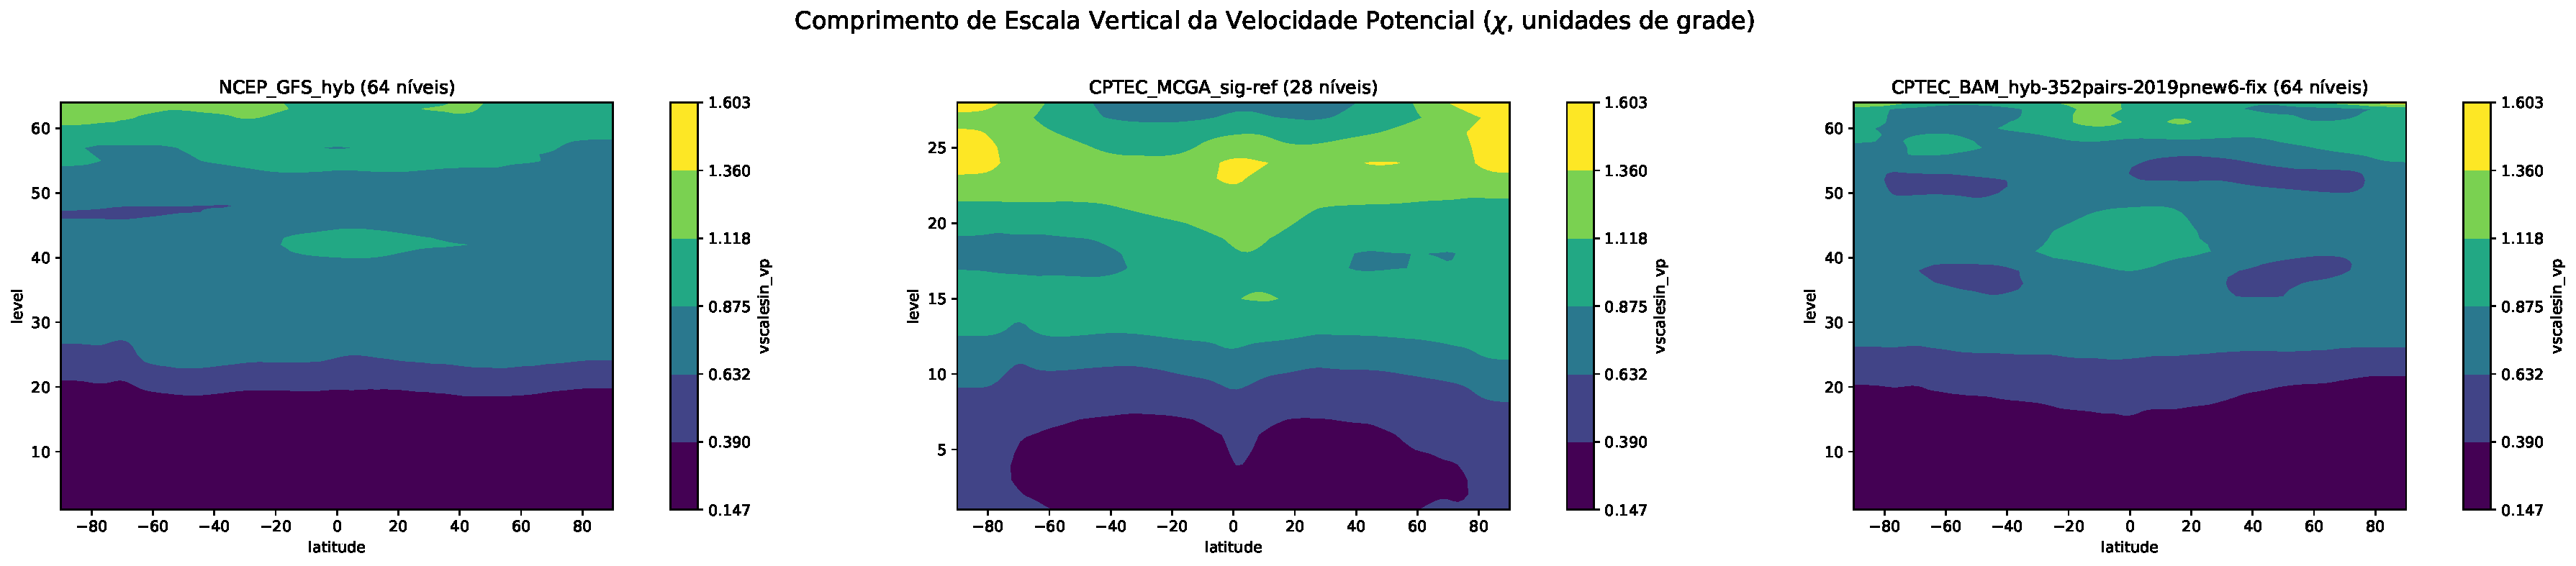
\includegraphics[width=1.\textwidth]{./figs/compara/vs_vp.pdf}
%%        \caption{Comprimento de Escala Vertical da $\chi$.}
%%    \end{center}
%%\end{figure}
%%\end{frame}
%
%\begin{frame}{Resultados}
%\framesubtitle{Comprimentos de Escala (Verticais)}
%\begin{figure}[H]
%    \begin{center}
%        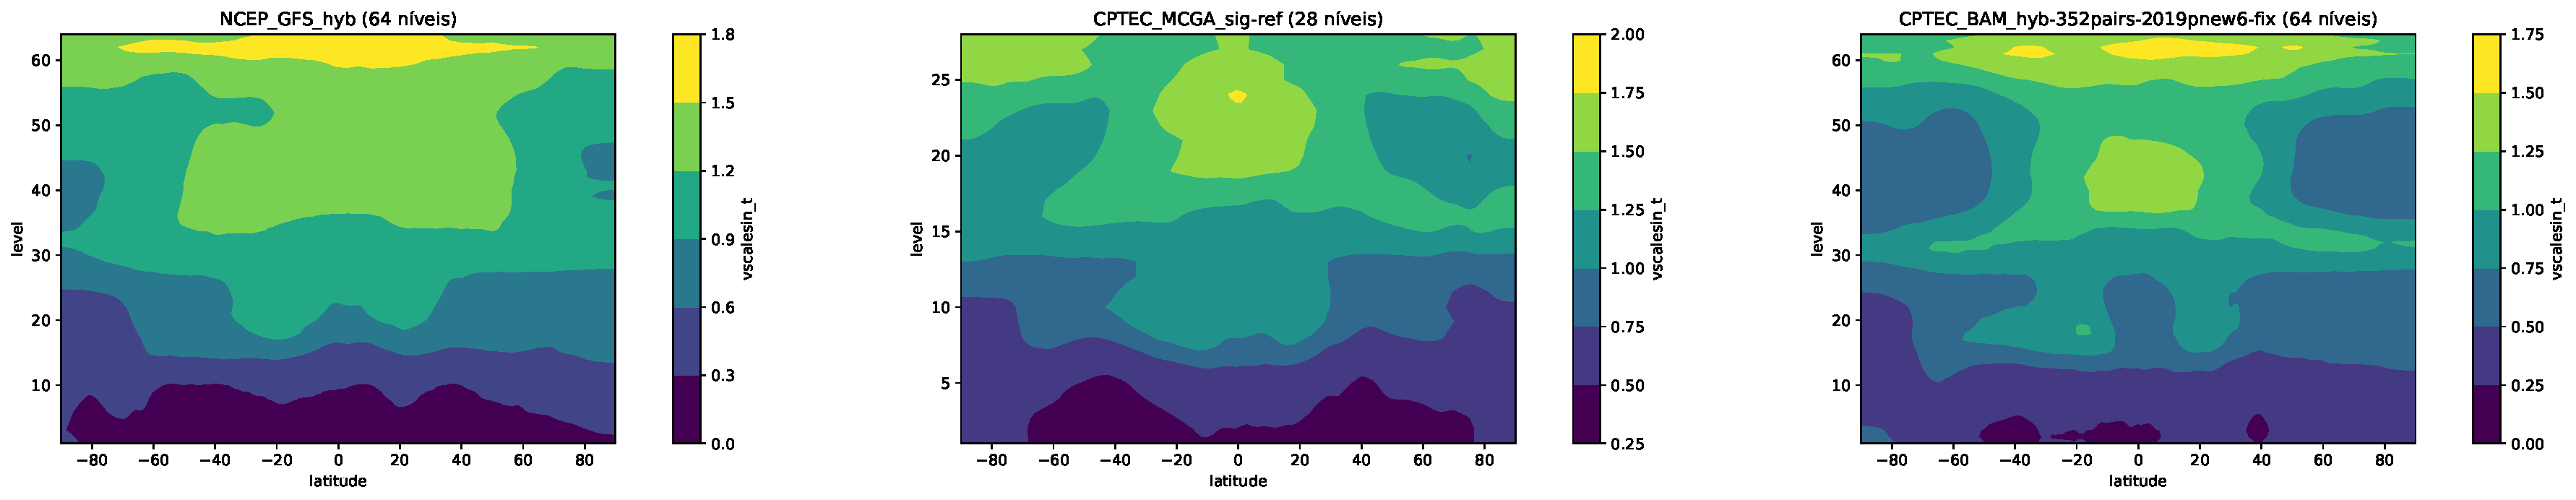
\includegraphics[width=1.\textwidth]{./figs/compara/vs_t.pdf}
%        \caption{Comprimento de Escala Vertical da $Tv$.}
%    \end{center}
%\end{figure}
%\end{frame}

\subsection{Exemplos Estruturas $\mathbf{B}$}

\begin{frame}{Resultados}
\framesubtitle{Exemplos Estruturas $\mathbf{B}$}
\vspace{-2em}
\begin{figure}[H]
    \begin{center}
        \hspace*{1em}\subfigure[Projeção da $\psi$ no nível 0 sobre o perfil da parte balanceada da $Tv$ ($Tv_{b} = \mathbf{G}\psi$).]{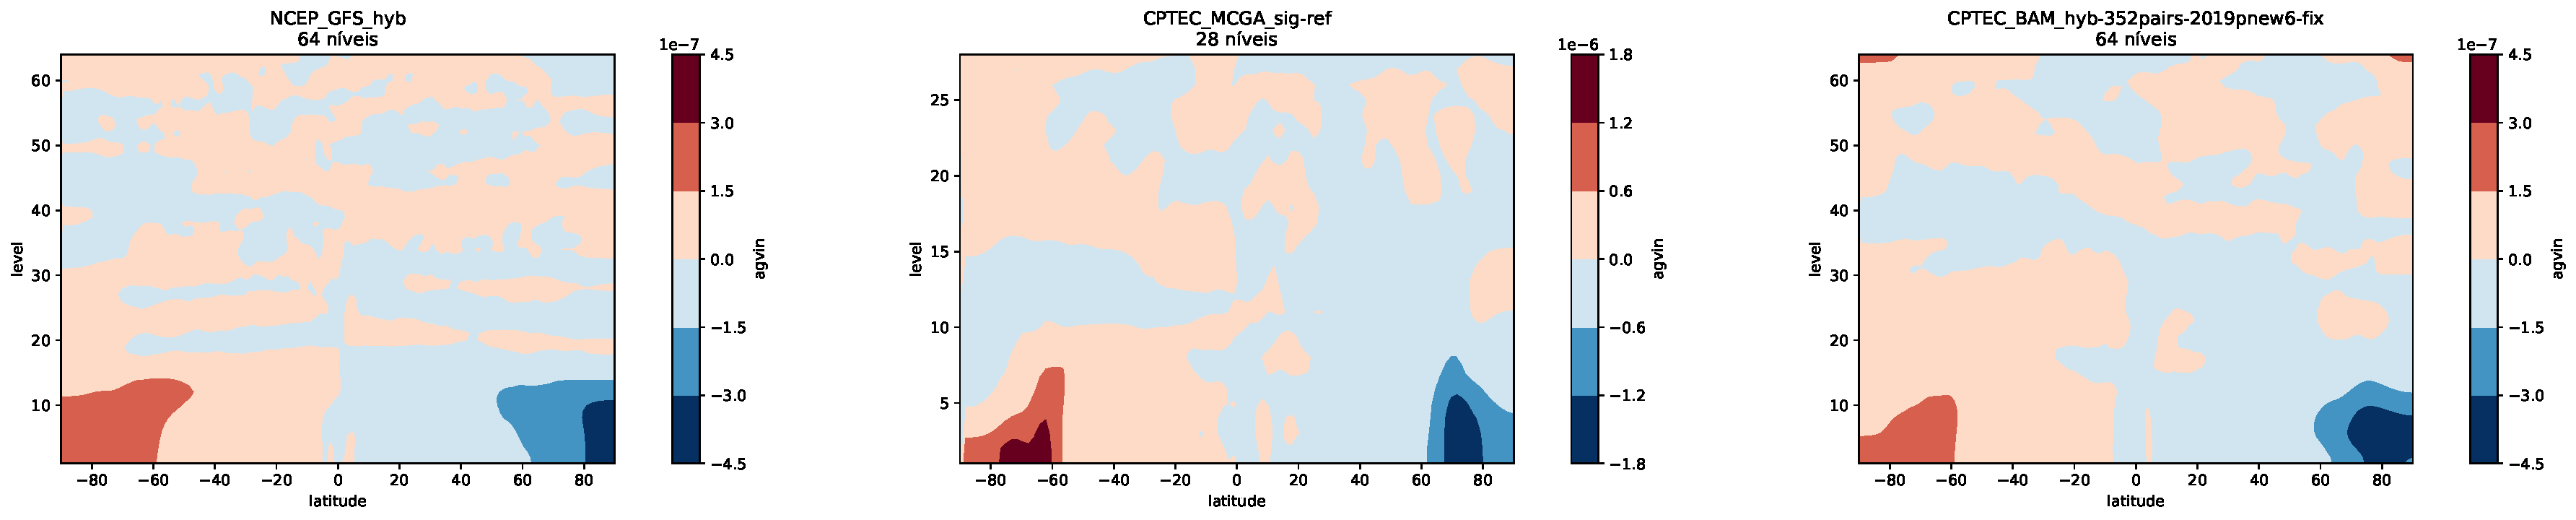
\includegraphics[width=1.\textwidth]{./figs/compara/agvin.pdf}} \\
        \hspace*{1em}\subfigure[Desvio-padrão da $Tv$.]{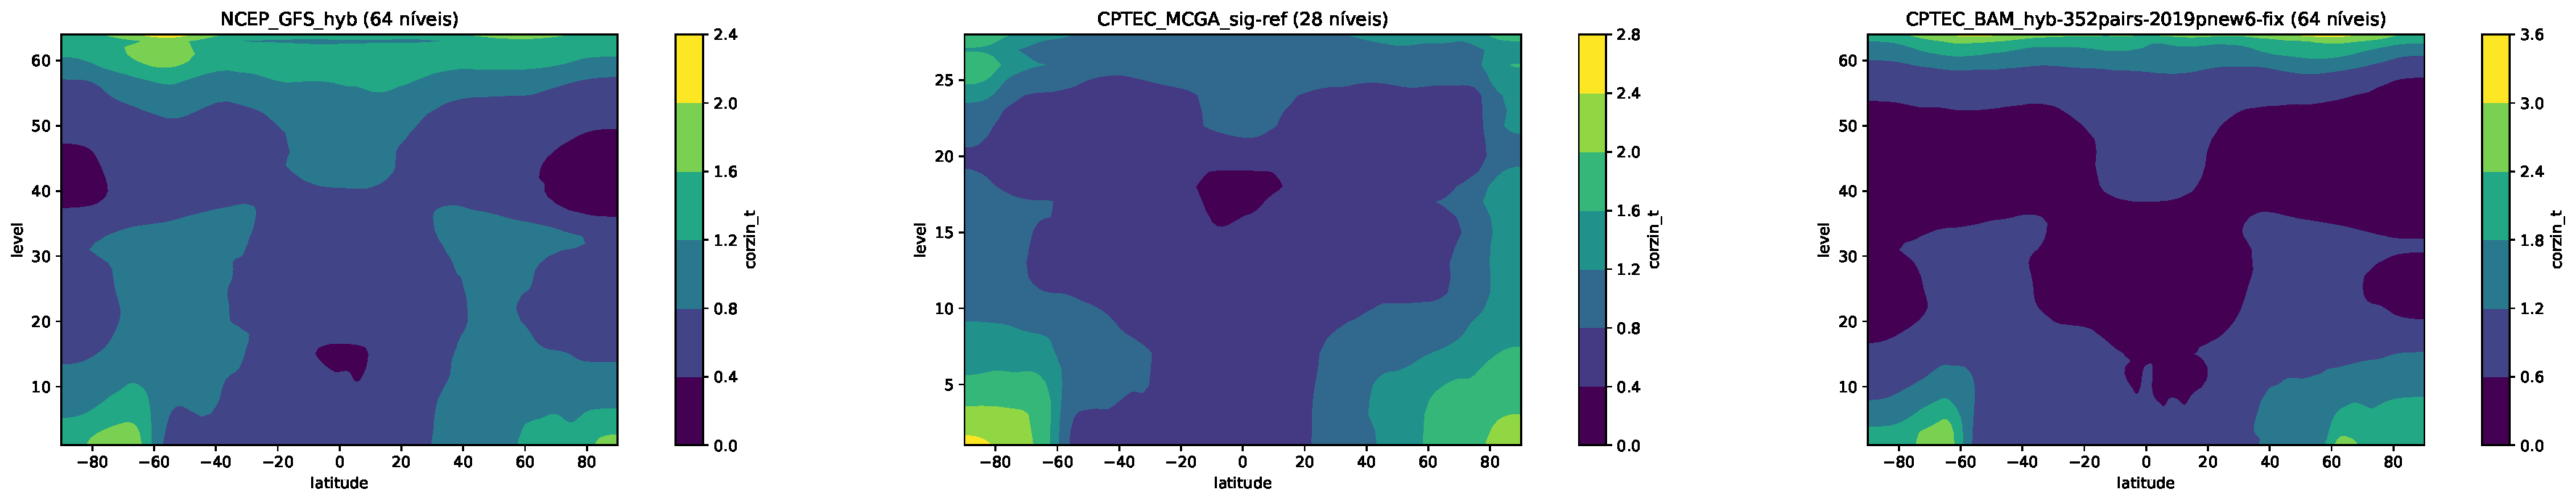
\includegraphics[width=1.\textwidth]{./figs/compara/t.pdf}}
        \caption{}
    \end{center}
\end{figure}
\end{frame}

\begin{frame}{Resultados}
\framesubtitle{Exemplos Estruturas $\mathbf{B}$}
\vspace{-2em}
\begin{figure}[H]
    \begin{center}
        \hspace*{1em}\subfigure[Comprimento de Escala Horizontal da $Tv$.]{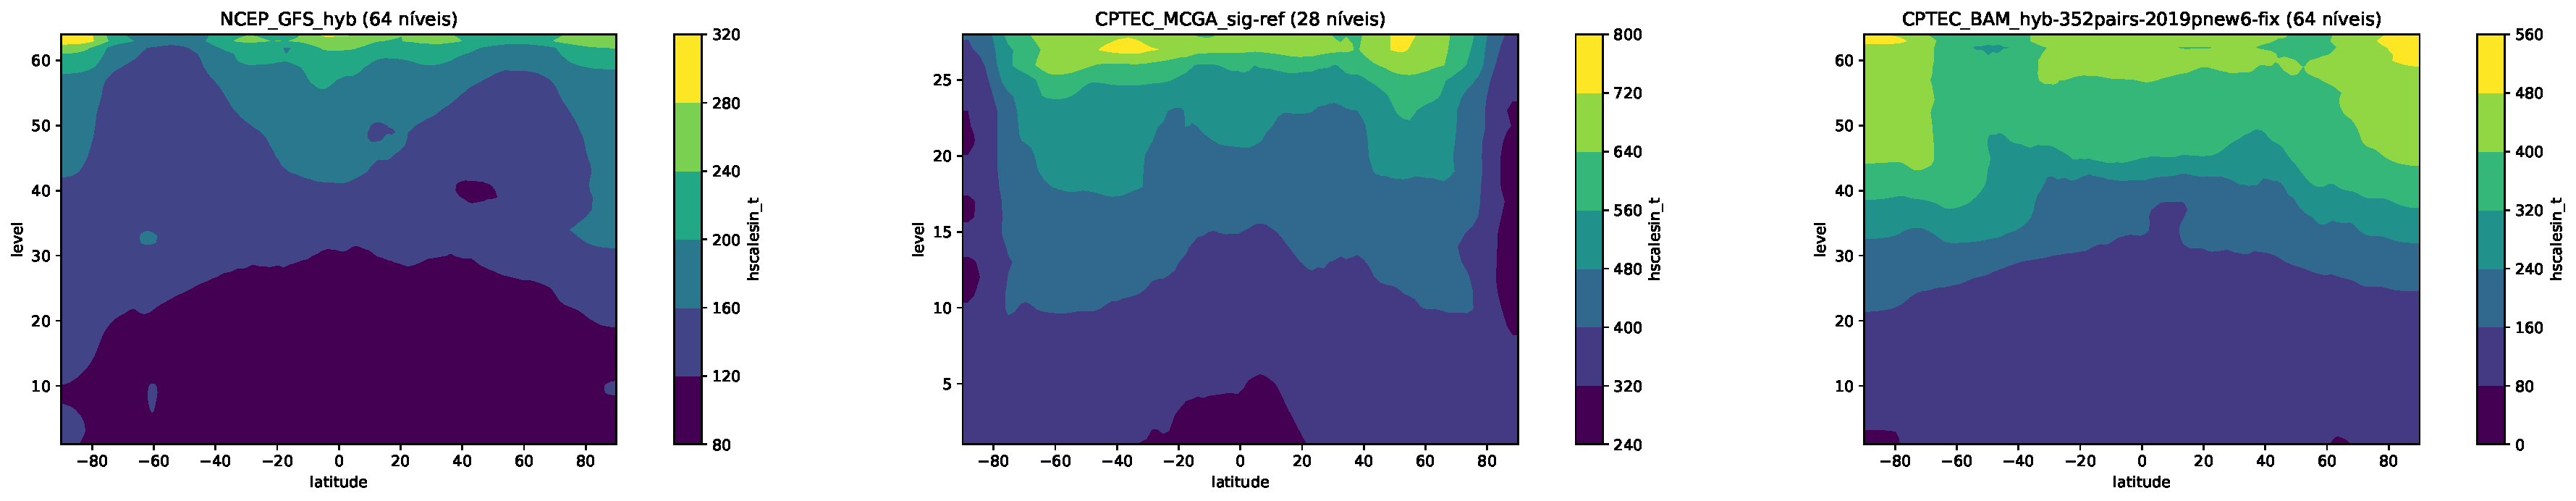
\includegraphics[width=1.\textwidth]{./figs/compara/hs_t.pdf}} \\
        \hspace*{1em}\subfigure[Comprimento de Escala Vertical da $Tv$.]{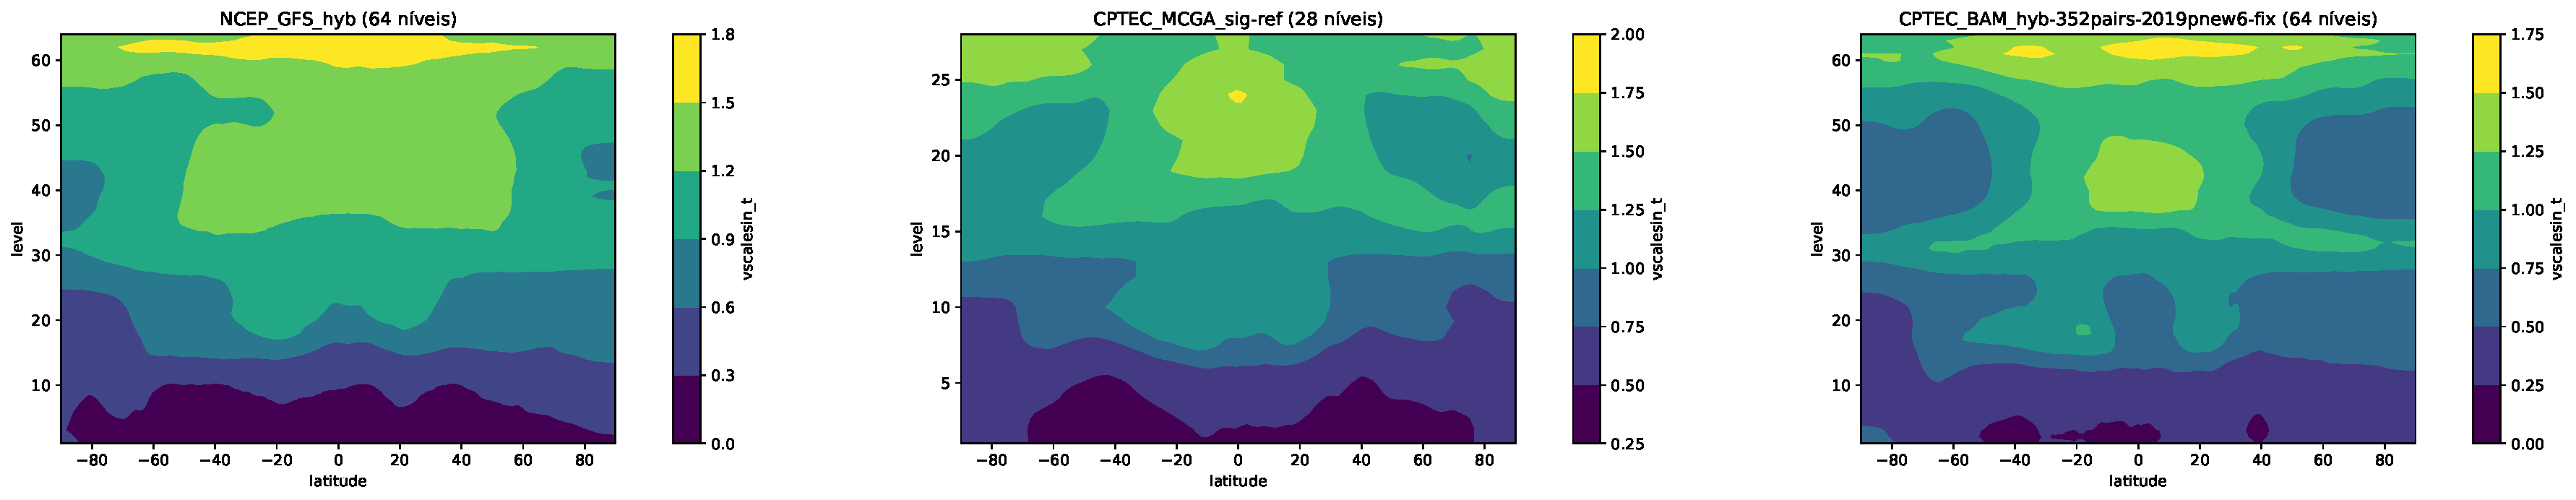
\includegraphics[width=1.\textwidth]{./figs/compara/vs_t.pdf}}
        \caption{}
    \end{center}
\end{figure}
\end{frame}

\subsection{Experimento Obs. Única}

\begin{frame}[fragile]{Resultados}
\framesubtitle{Experimento Obs. Única}
	\vspace{-2.5em}
	\begin{columns}
    	\begin{column}{0.35\textwidth} 
			\vspace{-3.75em}
			\begin{block}{Experimento Obs. Única:}
				\vspace{0.5em}
				Incrementos de $T$ em 1000 hPa. À esquerda $\mathbf{B}$ CPTEC e à direita, $\mathbf{B}$ NCEP (DTC). Para cada matriz, testou-se a opção anisotrópica \cite{bastarz/2017}.
			\end{block}
		\end{column}
		\hspace*{2em}
		\begin{column}{0.5\textwidth}
    		\begin{figure}[H]
      			\centering
		        \hspace*{-5.5em}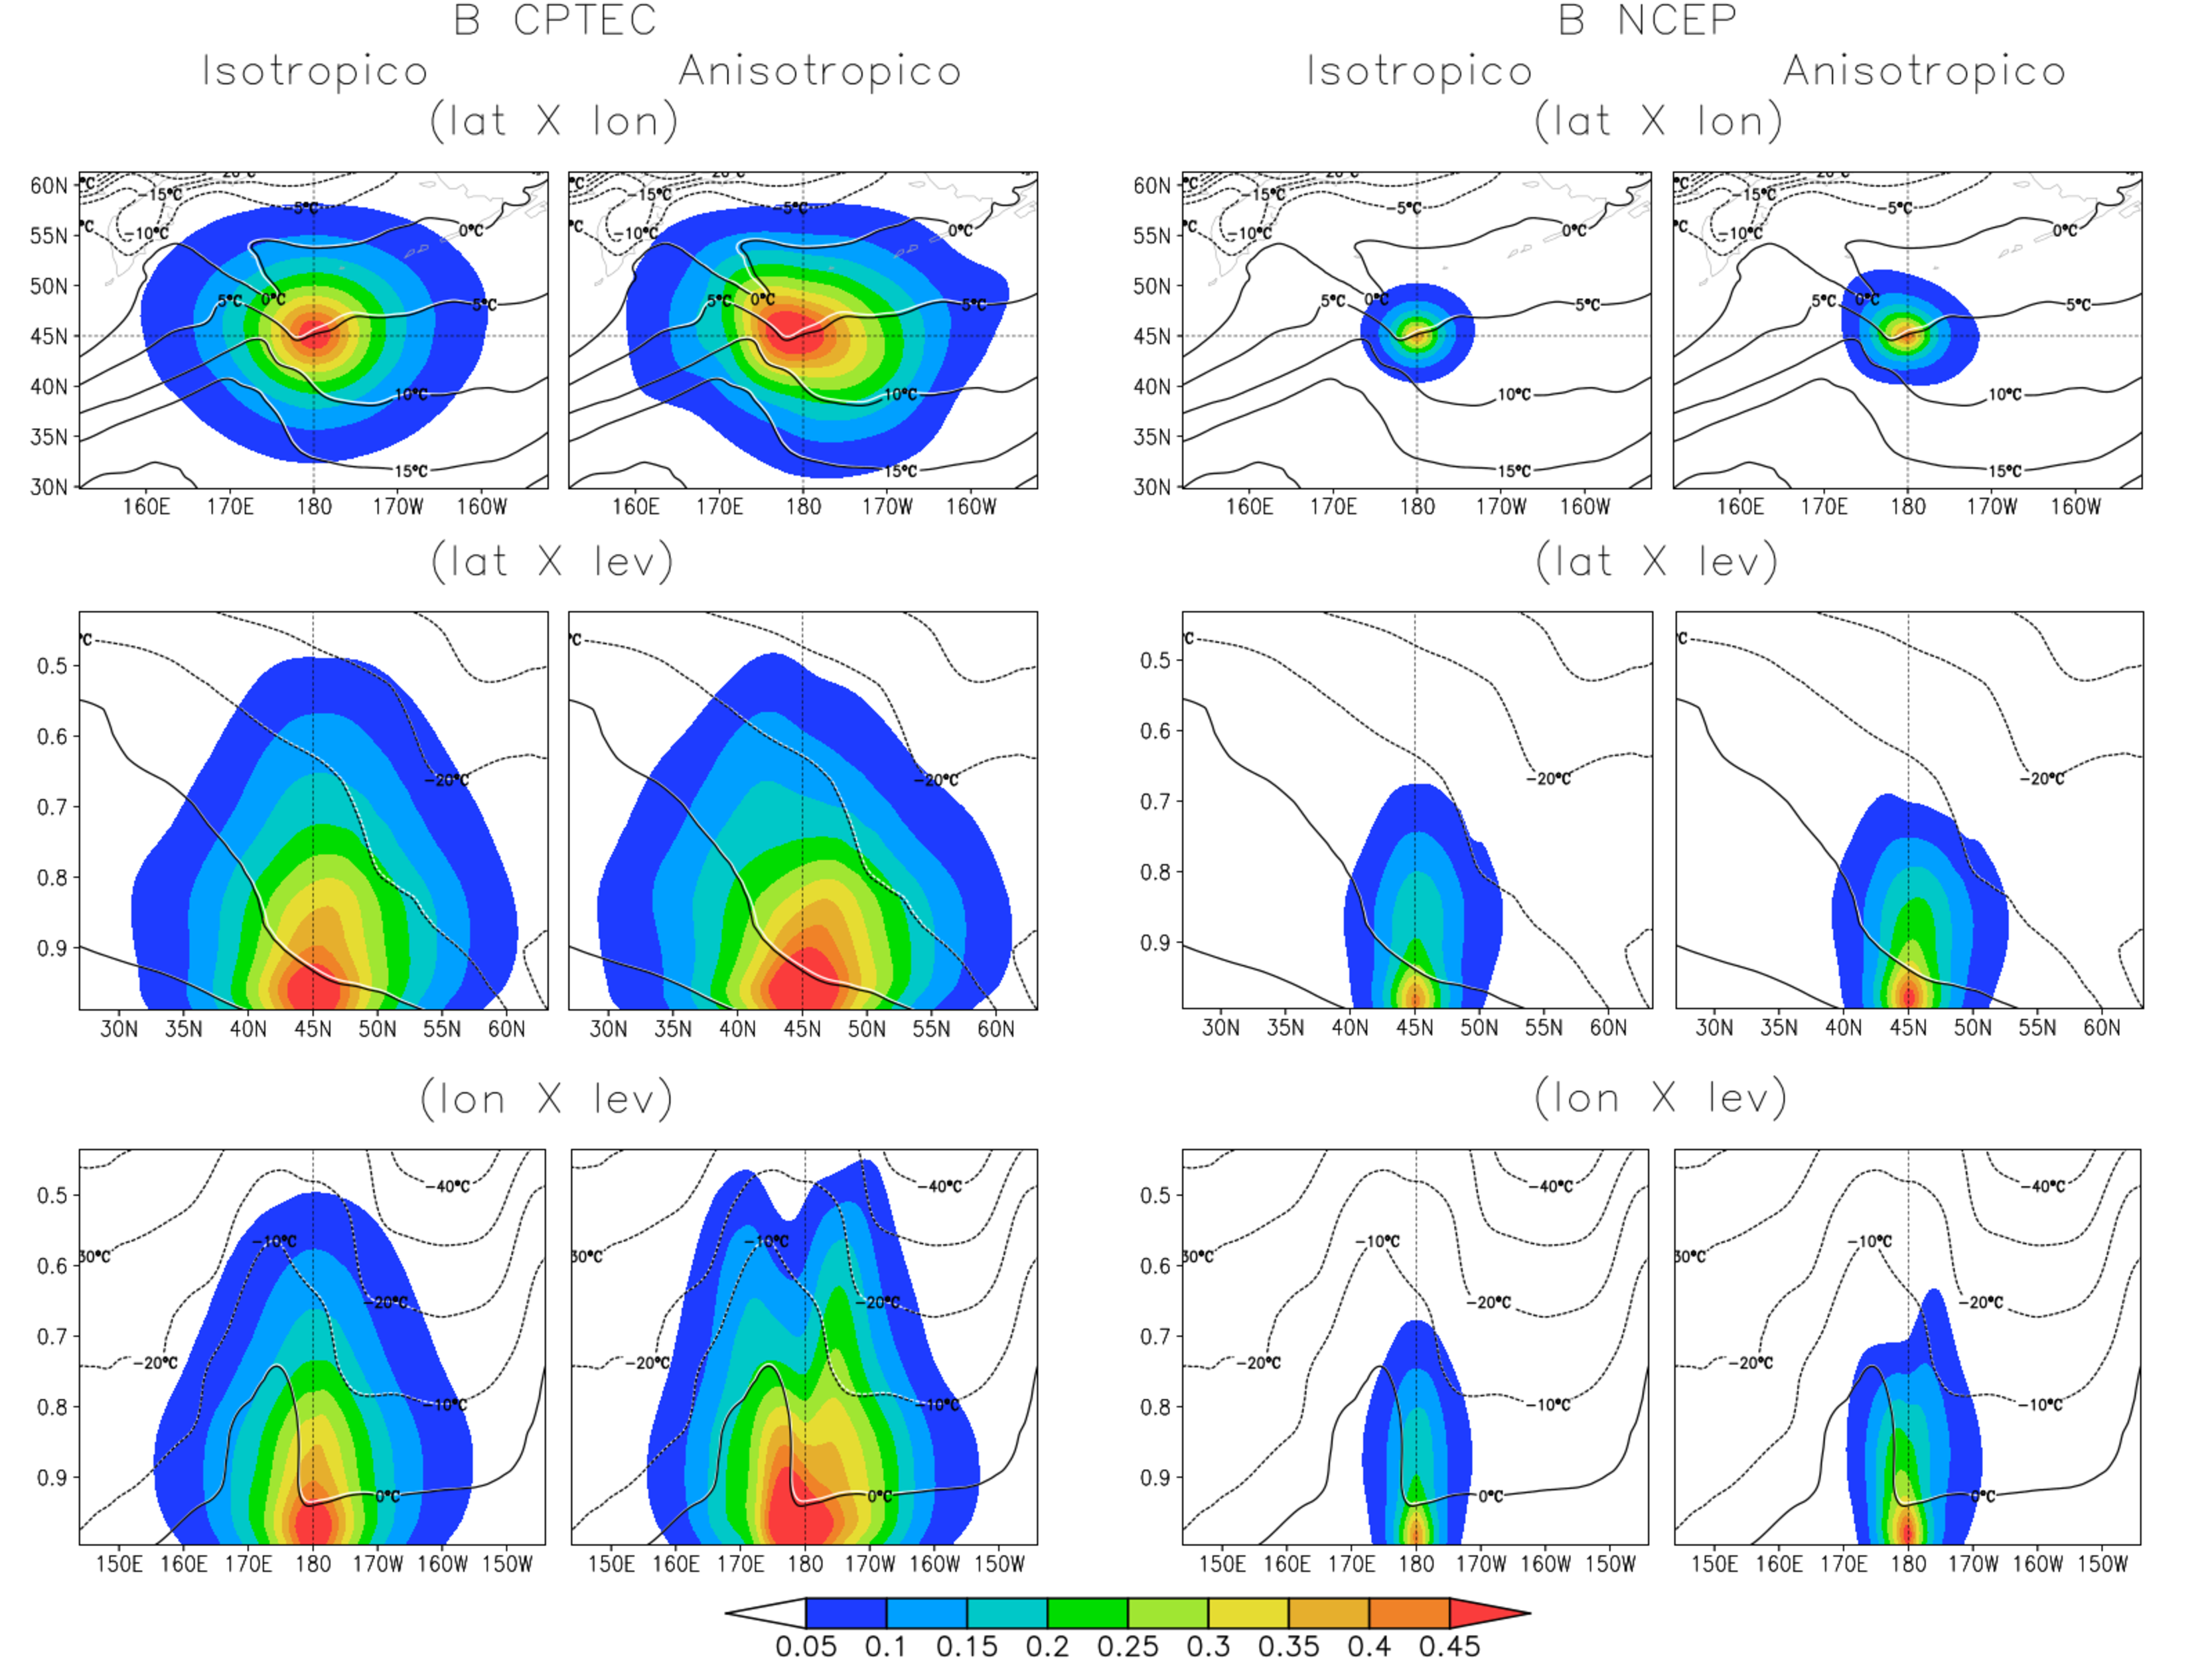
\includegraphics[trim={0 0 0 2.5cm},clip,scale=0.175]{./figs/fig5.pdf}
				\caption{}
			\end{figure}
		\end{column}
	\end{columns}
\end{frame}

%\subsection{Incremento de análise}

%\begin{frame}[fragile]{Resultados}
%\framesubtitle{Incremento de Análise ($\mathbf{B}\sigma$)}
%%  \metroset{block=fill}
%  %\vspace{-2em}
%  %\begin{block}{Aspecto do Incremento de Análise ($\mathbf{B}$ CPTEC):}
%    \vspace{-2em}
%    \begin{figure}[H]
%      \centering
%    %   \includegraphics[scale=0.09]{./figs/matrizB/incrementos_anl/incremento_analise_bcptec-crop.png}
%      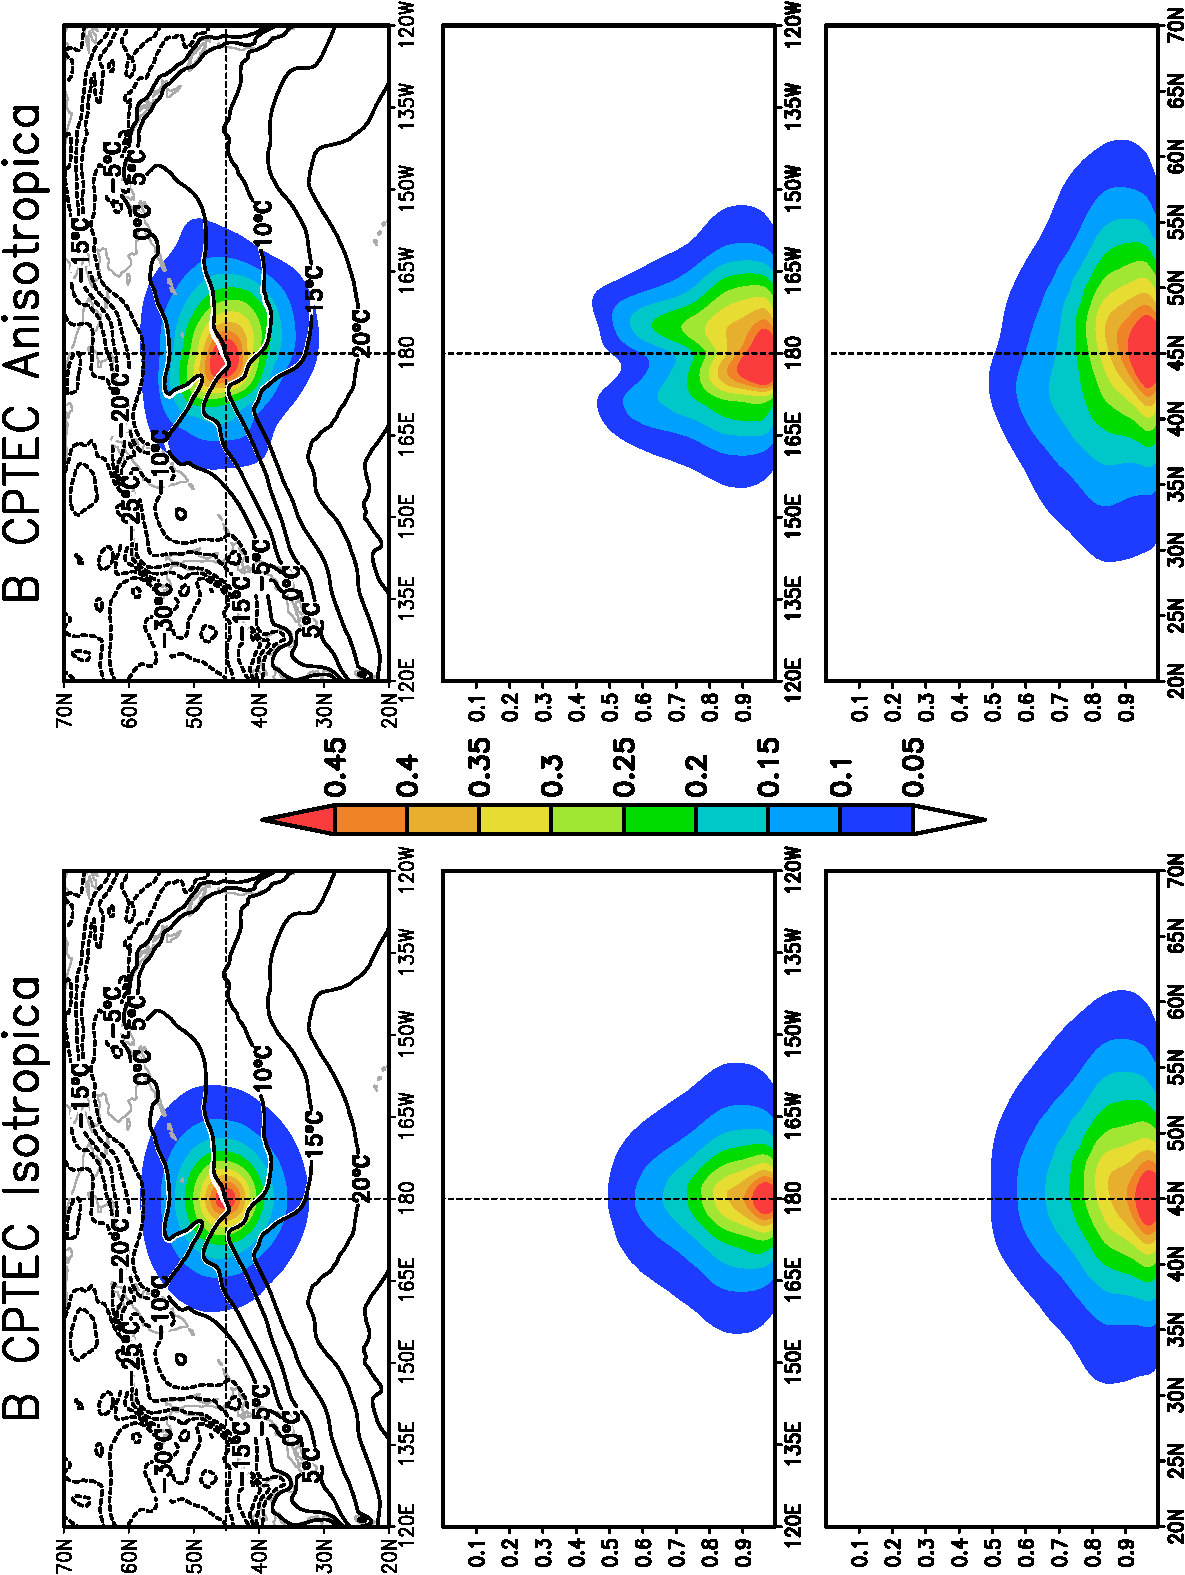
\includegraphics[trim={0.9cm
%      0 0 0},clip,scale=0.33,angle=-90]{./figs/incr_anl_t1000_Bcptec-artigo_rbmet-crop.pdf}
%      \caption{Esquerda: incrementos isotrópicos; direita: anisotrópicos \cite{bastarz/2017}.}
%    \end{figure}
%  %\end{block}
%\end{frame}

%\begin{frame}[fragile]{Resultados}
%\framesubtitle{Produção Técnica}
%	\vspace{-2.5em}
%	\begin{columns}
%    	\begin{column}{0.35\textwidth} 
%			\vspace{-3.75em}
%			\begin{block}{Incremento de Análise:}
%				\vspace{0.5em}
%				Incrementos de $T$ em 1000 hPa. À esquerda $\mathbf{B}$ CPTEC e à direita, $\mathbf{B}$ NCEP (DTC). Para cada matriz, testou-se a opção anisotrópica \cite{bastarz/2017}.
%			\end{block}
%		\end{column}
%		\hspace*{2em}
%		\begin{column}{0.5\textwidth}
%    		\begin{figure}[H]
%      			\centering
%		        \hspace*{-5.5em}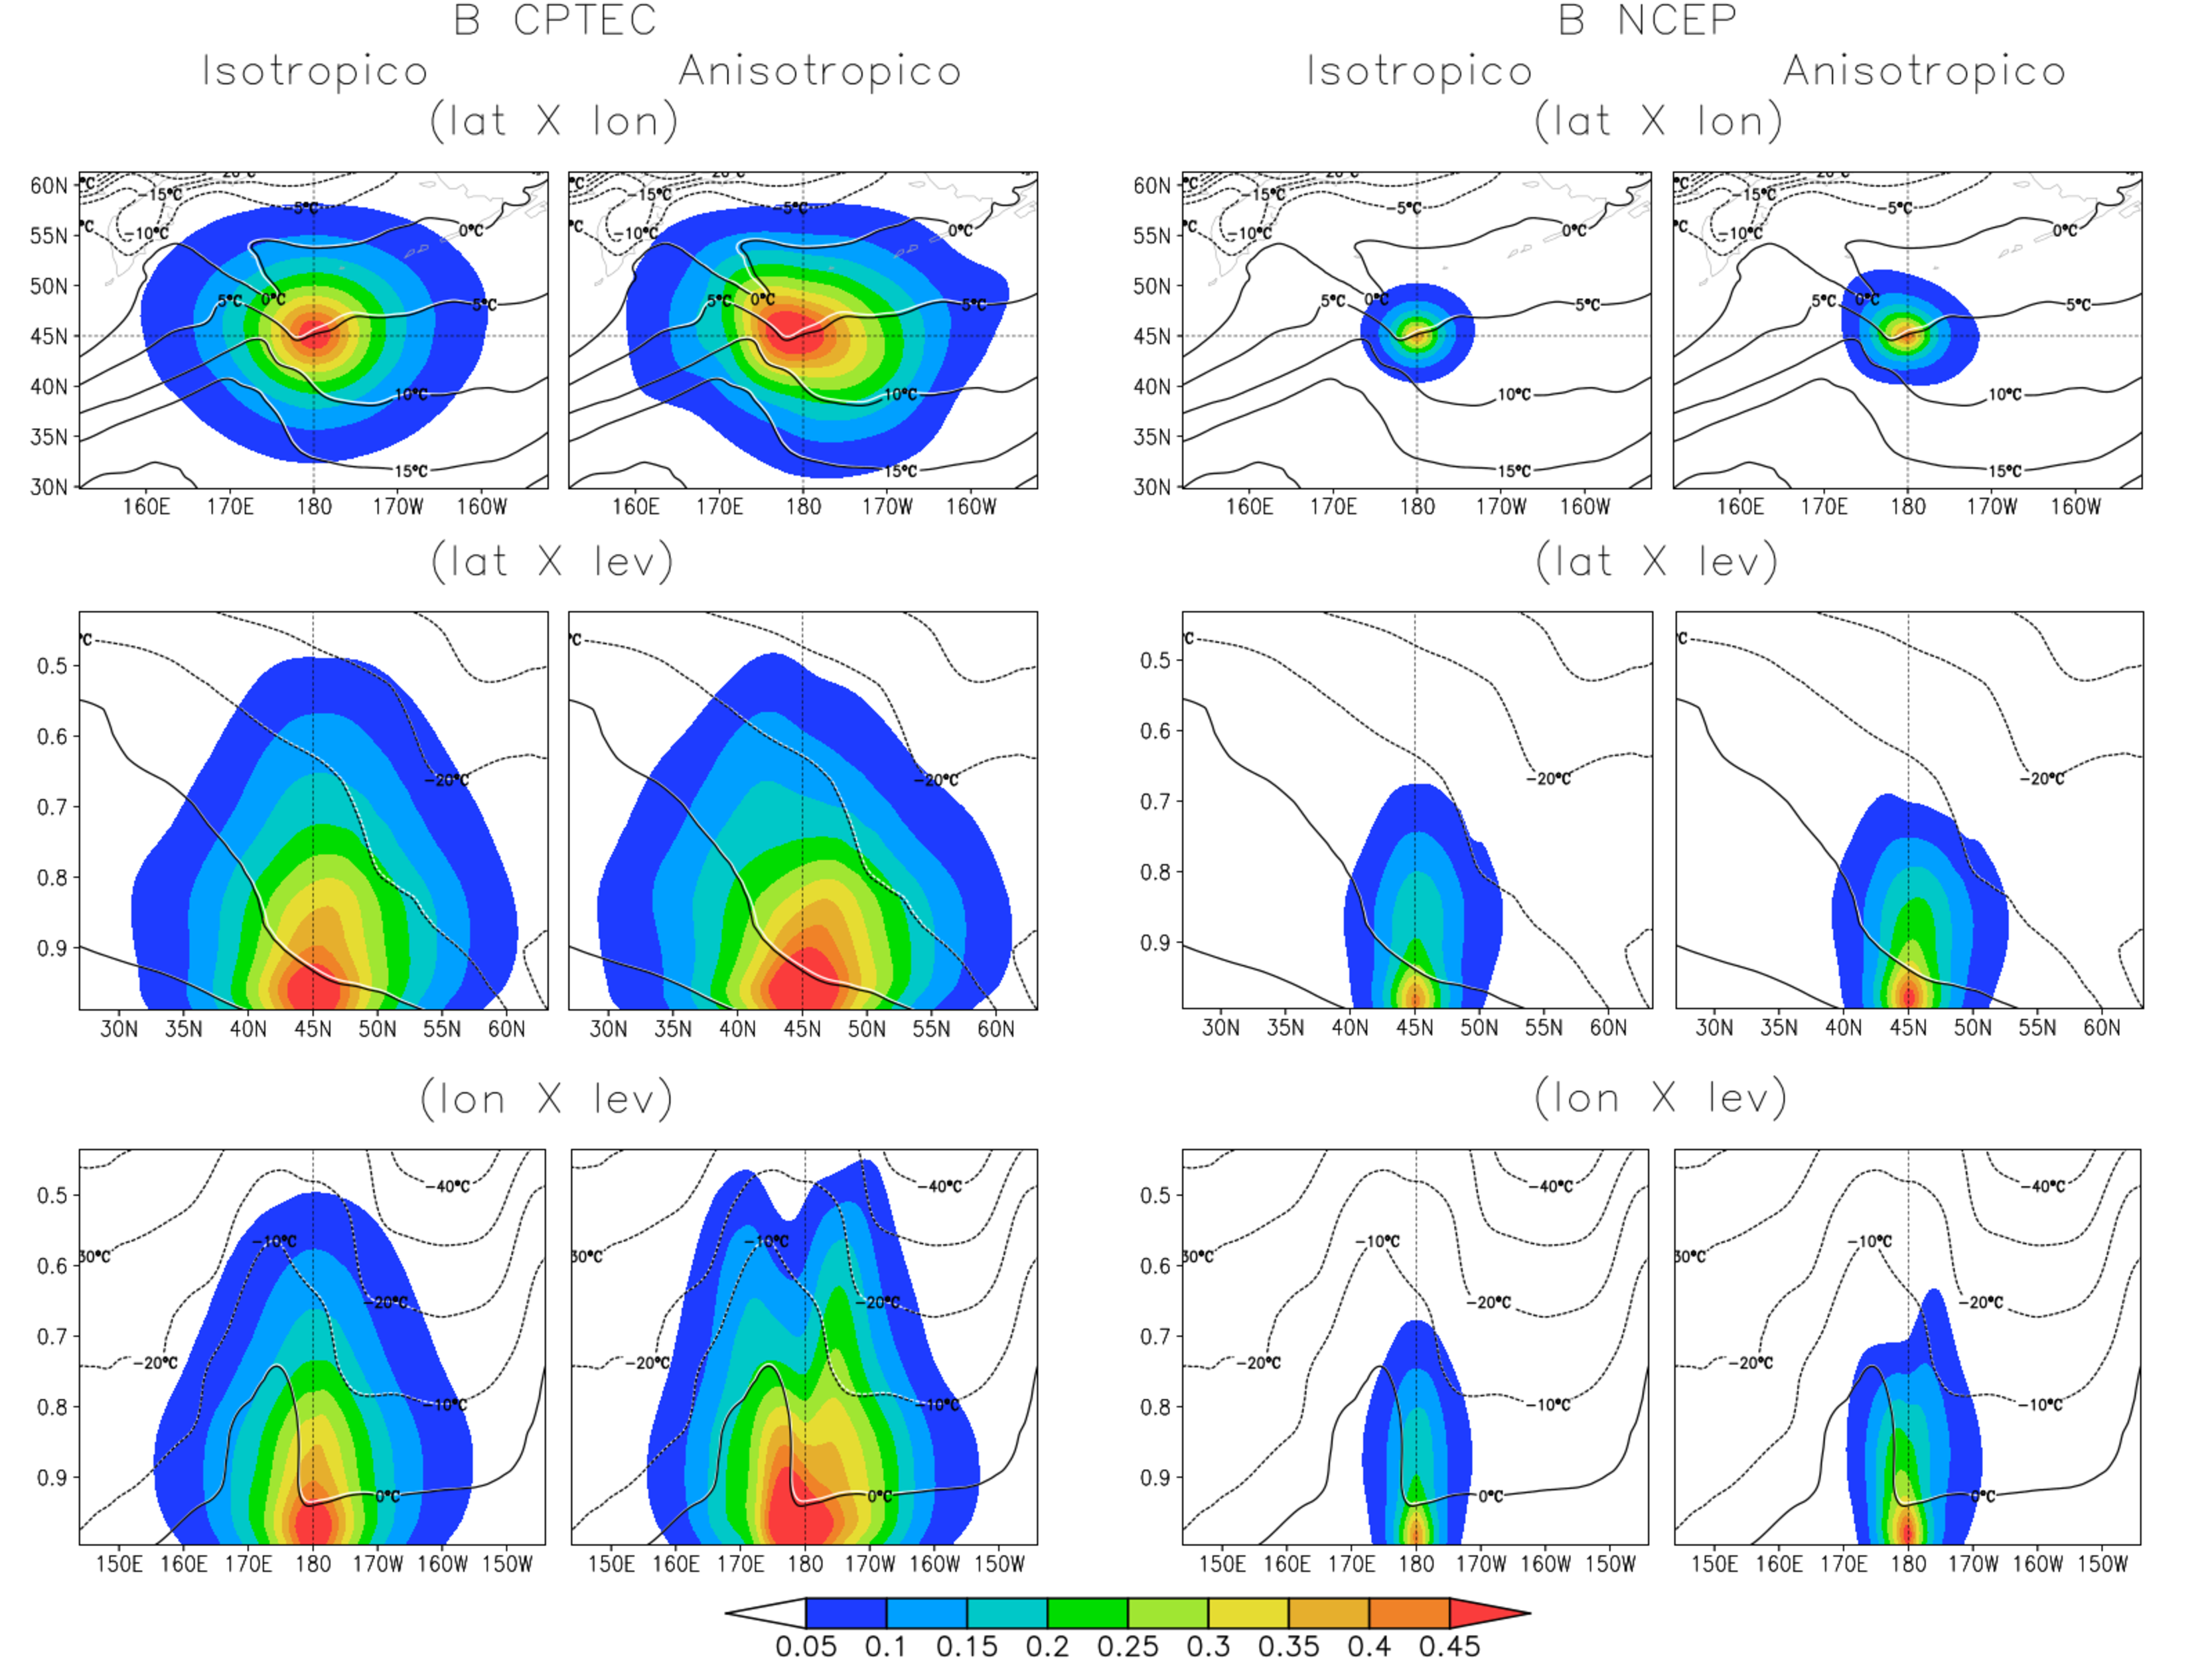
\includegraphics[trim={0 0 0 2.5cm},clip,scale=0.175]{./figs/fig5.pdf}
%				\caption{}
%			\end{figure}
%		\end{column}
%	\end{columns}
%\end{frame}

\section{MONAN}

\subsection{JEDI}

\begin{frame}[fragile]{MONAN}
\framesubtitle{JEDI \faJedi}
	\begin{block}{JEDI - \textit{Joint Effort for Data assimilation Integration}:}
	\vspace{0.5em}
    O \href{https://www.jcsda.org/jcsda-project-jedi}{JEDI} é composto de vários frameworks que implementam partes específicas do sistema de assimilação, por exemplo:
    \begin{itemize}
        \item \href{https://github.com/JCSDA/ioda}{IODA} - \textit{Interface for Observation Data Access};
        \item \href{https://github.com/JCSDA/ufo}{UFO} - \textit{Unified Forward Operator};
        \item \href{https://github.com/JCSDA/saber}{SABER} - \textit{System-Agnostic Background Error Representation};
        \pause
        \item Repositórios estão concentrados no \href{https://github.com/orgs/JCSDA/repositories}{GitHub do JCSDA} (\textit{Joint Center for Satellite Data Assimilation}).
    \end{itemize}
    \vspace{1em}
    \pause
    \begin{itemize}
    	\item \faUserGraduate~participação na 7$^{a}$ \textit{\href{https://www.jcsda.org/jedi-academies}{JEDI Academy}}, de 4-8 de Outubro de 2021 (online, João e Carlos).
    \end{itemize}
	\end{block}
\end{frame}

\subsection{SABER}

\begin{frame}[fragile]{MONAN}
\framesubtitle{SABER \faRebel}
	\begin{block}{SABER - \textit{System-Agnostic Background Error Representation}:}
	\vspace{0.5em}
    O SABER implementa o \href{https://github.com/benjaminmenetrier/bump-standalone}{BUMP} (\textit{Background error on Unstrucured Mesh Package}), que é uma biblioteca F90 onde estão disponíveis os métodos de cálculo da matriz $\mathbf{B}$:
    \begin{itemize}
        \item Funciona em qualquer grade (gaussiana, esférica-cubada, não-estruturada, oceânica, área limitada);
        \item Trabalha em grade mais grosseira, pois em geral, as estruturas representadas pela matriz de covariância são maiores do que a grade do modelo.
    \end{itemize}		
	\end{block}
\end{frame}

\section{Dificuldades e Desafios}

\subsection{Algumas Questões}

\begin{frame}{Dificuldades e Desafios}
\framesubtitle{Algumas Questões \faQuestionCircle}
    \begin{itemize}
        \item Precisamos sempre atualizar a matriz $\mathbf{B}$? Com que frequência?
        \pause
        \item É necessário uma grande quantidade de pares de previsão? Qual é a quantidade ideal que representa adequadamente a variabilidade espaço-temporal dos erros do modelo?
        \pause        
        \item A matriz $\mathbf{B}$ precisa estar na mesma resolução horizontal que o modelo operacional (na vertical sim!)?
        \pause        
        \item Para a operação: tratamento de $sst$, $oz$ e $cw$;
        \pause        
        \item Uma forma de atualizar a matriz $\mathbf{B}$ é através de um sistema que envolva o ensemble (e.g., 3DEnVar) ou mesmo o 4DVar;
        \pause        
        \item Uma média móvel pode ser uma alternativa para o caso 3DVar ou mesmo o 3DEnVar?
        \pause        
        \item Para o \textbf{MONAN}: não necessariamente todas as covariâncias são/serão tratadas da mesma forma (superfície terrestre pode ser mais simples do que a atmosférica - isso depende da complexidade da componente e do próprio sistema de assimilação de dados).
    \end{itemize}
\end{frame}

\section{Referências Bibliográficas}

\begin{frame}
\frametitle{Referências Bibliográficas}
\framesubtitle{\faBookOpen~\faCode~\faPython}
\vspace{-1.5em}
\small\bibliography{referencias}
\end{frame}

% Frame Final (NÃO MODIFICAR)
\usebackgroundtemplate%
{%
	
\includegraphics[width=\paperwidth,height=\paperheight]{fundo_slide_inpe_sem_logo.png}%
}

\begingroup
\setbeamertemplate{footline}{}
{\nologo
\begin{frame}
	\begin{figure}[H]
    	\vspace{-4em}
		%\begin{center}
		\centering
        	\hspace*{1.5em}
\includegraphics[width=1.\textwidth]{DesinacaoNominativaCentralizada2020.pdf}
    	%\end{center}
	\end{figure}
\end{frame}
}
\endgroup

\end{document}
